\documentclass[11pt]{asu}

\usepackage[]{graphics}
\usepackage{graphicx}
\usepackage{setspace}
\usepackage{lscape}
\usepackage{rotating}
\usepackage{listings}
\usepackage{url}
\usepackage{courier}
\usepackage{csquotes}
\usepackage{fixltx2e}
\usepackage{xinttools}
\usepackage[]{algorithm2e}
\usepackage[toc,page]{appendix}

\newcounter{bitindex}

\clubpenalty=5000
\widowpenalty=5000
\renewcommand\lstlistlistingname{List of Listings}
\setlength{\belowcaptionskip}{.25in}

%c++ listing box settings
\lstset{language=C++,
	numberstyle=\footnotesize,
	basicstyle=\ttfamily\footnotesize,
	morekeywords={uint8_t, uint16_t, uint32_t, uint64_t},
	numbers=left,
	stepnumber=1,
	frame=single,
	breaklines=true,
  showstringspaces=false
}

%create image of a float showing each bit
\newcommand{\floatimage}[3]{%
  \setlength{\unitlength}{1mm}
  \setlength{\fboxsep}{0mm}
  \begin{picture}(130,16)
    % sign bit
  \put(2,4){\framebox(4,8){#1}}
  % exponent
  \setcounter{bitindex}{1}%
  \xintFor* ##1 in {#2}
  \do
  {\put(\numexpr 2+4*\value{bitindex},4){\framebox(4,8){##1}}%
   \stepcounter{bitindex}}%
  % fraction
  \setcounter{bitindex}{1}%
  \xintFor* ##1 in {#3}
  \do
  {\put(\numexpr 34+4*\value{bitindex},4){\framebox(4,8){##1}}%
   \stepcounter{bitindex}}%
  % upper labels
  \put(0,14){\scriptsize{MSB}}
  \put(126,14){\scriptsize{LSB}}
  %lower labels
  \put(3,0){\scriptsize{S}}
  \put(7,0){\line(0,1){2}}
  \put(7,1){\vector(1,0){8}}
  \put(16,0){\scriptsize{Exponent}}
  \put(37,1){\vector(-1,0){8}}
  \put(37,0){\line(0,1){2}}
  \put(39,0){\line(0,1){2}}
  \put(39,1){\vector(1,0){38}}
  \put(79,0){\scriptsize{Fraction}}
  \put(130,1){\vector(-1,0){38}}
  \put(130,0){\line(0,1){2}}
\end{picture}%
}

%inline code command, using courier font
\newcommand{\code}[1]{\texttt{#1}}

\title{Conlangtionary: Prototyping a Language-Agnostic Dictionary for the Web}
\degree{Bachelor of Science}
\department{Computer Science}
\gradmonth{May}
\gradyear{2016}
\author{Christopher Waldon}  
\thesischair{E. Frank Barry}
\thesismemberone{Donna Lillian, Ph.D.}
\thesismembertwo{Dee Parks, Ph.D.}
\deptchair{Ted Zerucha, Ph.D.}
\dean{Dean}

\begin{document}
	\begin{preliminary}
		\maketitle
        \makecopyright
        \begin{abstract}
This project documents a prototype system that represents spoken languages of arbitrary structure or complexity for use by field linguists and conlangers. The prototype is capable of representing complex languages, but serves only as a foundation for future work, as it lacks many generative features that would make it appealing to its target audience.
\end{abstract}

		\tableofcontents
        \listoftables
        \listoffigures
        %\lstlistoflistings
	\end{preliminary}

	\newlinestretch{2}

		\begin{doublespace}
	    \chapter{Introduction}
\label{chap:introduction}

Conlangtionary exists to solve a very specific problem: storing a language in a web platform (as a dictionary and grammar) in such a way that you could theoretically represent any spoken language. Why does this problem matter? Many existing online dictionary services (e.g. Wiktionary \cite{Wiktionary}) make assumptions about the language that you are working on. Namely, they assume that the language already exists or that it is relevant to the entire online community. While these may seem like good assumptions, they actually hinder the platform's usefulness to two audiences: field linguists and ``conlangers".

Field linguists are simply researchers working to profile and preserve obscure spoken languages \cite{Field-linguistics}, but conlangers require more explanation. Conlanging is the hobby of inventing languages. To put it in more eloquent terms:

\begin{quote}
Conlanging is to linguistics what painting is
to art history, or hacking to computer science.
It’s a way of directly playing with language—
sometimes just for fun, and sometimes to test
out a new theory about how language works
with the mind. \cite{Conlanging-101}
\end{quote}

People conlang for many reasons. Authors often create languages for fictional worlds. TV shows and movie productions have recently started to hire conlangers to create the fictional languages for their worlds. Marc Okrand is best known for creating the Klingon language, but he has also created other languages commercially such as the Atlantean language for Disney's Atlantis. His success, and the success of others like him, has inspired many people to dabble in language creation. These cells of conlangers find one another through the internet, often via reddit's /r/conlangs or the Language Creation Society's listserv, and they build communities dedicated to sharing languages and techniques for their creation. At the time of this writing, reddit's conlanging community numbers 9,098 members. These communities share their languages online with platforms like Wikipedia that, while free and open-source, ultimately hinder their efforts by forcing users to create a page for each word and to manually enter a lot of information. Entering data in this way is tedious, and the results of such effort only serve to demonstrate how such a page-per-word format is ill-suited to the task of representing language.

To be clear, there are software tools such as PolyGlot for developing conlangs, but none of them are accessible as web applications. They force users to develop in a desktop environment, which makes it much harder for conlangers to share their languages with others or to collaborate on a common set of files. Conlangtionary is an effort to change that.

Chapter~\ref{chap:description} describes the design and intentions of the model that the project uses to store and manage user-created languages.

Chapter~\ref{chap:implementation} discusses the technologies and frameworks used to create Conglangtionary and explains why they were chosen.

Chapter~\ref{chap:usage} walks through using the Conlangtionary platform to create a language.

Chapter~\ref{chap:future} suggests improvements for future researchers to make the platform more useful.

Chapter~\ref{chap:conclusion} summarizes the project.
	    \chapter{Description}
\label{chap:description}
There are many design considerations when one is creating a web application with maximum flexibility. It is easy to make an assumption about how users will want to structure their data, and that assumption may unintentionally limit the capabilities of the software as a whole. Originally, Conlangtionary's design included features that tracked a definition's part-of-speech, but further consideration revealed that this design would limit conlangers to using parts of speech as a fundamental lexical category in their languages. This original design was refined for several months before arriving at the structure that the platform currently uses to store languages. Ultimately, the structure of Conlangtionary's data model can be broken down into three subsections: Language Representation, Language Generation, and Access Control.

\section{Language Representation}
\label{sec:language-representation}

Representing the internal structure of a language as data is difficult. It might be intuitive to break a language into words and to make each world have attributes like parts of speech and tense, but it is also extremely restrictive. By doing so, you limit the ways in which a word can be categorized. The concept of a ``part of speech" is simply a role that grammarians assign to a word, rather than an absolute law of linguistics. To allow adequate flexibility for the conlanging user, a different structure is necessary.

\subsection{Words}
\label{subsec:words}
In languages that have a written form, a word is a sequence or ``string" of characters conveying a pronunciation and meaning. However, a single word can have more than one definition. Consider the English word ``cleave." Cleave means both ``to adhere firmly and closely or loyally and unwaveringly" and ``to separate into distinct parts and especially into groups having divergent views," and it is thus the only English word to be its own antonym \cite{Merriam-Webster:cleave}. Clearly, any flexible language design needs to accommodate the overloading of a word by allowing multiple definitions. Since words can also have definitions with differing parts of speech (e.g. ``to go on a walk" where ``walk" is a noun, and ``I walk" where ``walk" is a verb), a reasonably flexible design must store data about the usage of a word at the definition level as well. This leaves little more than the string of characters that form a word to be stored at the word level, and instead puts most information into definitions.

\subsection{Definitions}
\label{subsec:definitions}
A word's definition needs to have several components: a fragment of text explaining that word's meaning, a pronunciation guide of some sort, an association with the word that it defines, and information about how to use this definition in context. The fragment explaining its meaning can be as simple as ``this word means tree" or as complex as ``[the] continuous surface of the body ... that begins with the inside flesh of the fingers and continues over the palm of the hand and up the inner side of the arm to the bend of the elbow" \cite{native-tongue}. Pronunciation guides vary between languages, but often a string in the International Phonetic Alphabet suffices.

The most challenging element of designing a definition is storing information about its grammatical role. The most naive way would be to allow a paragraph explaining proper usage to readers, but this is both cumbersome and difficult to parse. Searching by such information would require users to be perfectly consistent in formatting or messy keyword searches. However, the obvious alternative of hard-coding a part of speech, tense, declension, aspect, or any other obscure lexical category leaves the conlanger unable to invent meaningful categories for their definitions that can then be expressed by the application. To solve this problem, Conlangtionary uses tags on definitions to store data.

\subsection{Tags}
\label{subsec:tags}
Readers will no doubt be familiar with the kinds of tags that are used to categorize blog posts or tweets. Conlangtionary employs a similar system to organize definitions according to how they function within a language. Since a given definition can have any number of tags, it follows that those tags are capable of placing that definition into any number of sets of words with the same tag. This means that tags can be used for every level of meaningful differentiation within a language.

For instance, if a user were defining the English language in Conlangtionary, they might create a word ``walk" with multiple definitions. Walk could be tagged as a ``Noun" if the user were simply tagging by English parts of speech, but that fails to leverage the full power of the tagging system. Walk could also be tagged as ``Singular," ``Regularly Pluralized," and ``Quantitative." These could mean, respectively, that the word is currently in a singular form, that it follows the usual English pluralization rule (namely, adding an ``s" suffix) and that it can be used grammatically with a quantity. The last is important because words that refer to substances often cannot be used in this way. For instance, one cannot say ``I have two rice and eighteen water" without context.

Tags are also extremely useful when it comes to Conlangtionary's generative features (see section \ref{sec:language-generation}).

\subsection{Descriptions}
\label{subsec:descriptions}

A language description is by far the simplest component of a Conlangtionary language. A Description is a markdown description of the language and its use \cite{Markdown}. It has no length limit, and it is intended to describe the culture, origin, pronunciation, and grammar of the language. Since it is in the markdown format, it can easily hyperlink to external resources on the language, which is the preferred way to include reference materials.

\subsection{Structure Summary}
\label{subsec:structure-summary}

To put all of the components together, a Conlangtionary language is a markdown description, a collection of words, and a collection of tags. Each word in the language has many definitions and each of those definitions has many tags. This loose structure allows the language creator to define arbitrarily complex categories for their language without encountering limits mistakenly imposed by the application developer. Ultimately though, representing a language doesn't make Conlangtionary any more useful than a digital notebook. The generative features of the platform are what allow it to actually surpass its pen-and-paper counterparts.

\section{Language Generation}
\label{sec:language-generation}

Asking a digital system to understand a completely arbitrary grammar is a hard problem, which is why Conlangtionary--in its current incarnation--makes no attempt whatsoever to comprehend language grammar. However, Conlangtionary does understand regular expressions, and it is able to use these regular expressions to generate new vocabulary based on certain inputs.

This feature was key in differentiating a platform like Conlangtionary from something like Wiktionary. Wiktionary tries to include all conjugations/declensions/pluralizations of a given word on that word's page, but these entries must always be entered by hand. This process is tedious, time-consuming, and error-prone. It seems like a platform with the data-manipulation capabilities of a modern computer should be able to handle such transformations automatically, provided that they follow rules. This is what Conlangtionary offers in its Morphological Generator feature.

\subsection{Tag-based Generation}
\label{subsec:tag-based-generation}

As a simple example of how to leverage the Morphological Generator, consider the English verb ``walk." An assidious conlanger profiling English could have tagged it with the following: ``Verb," ``First-Person Singular," ``Present-Tense," and ``Regular-Conjugation." With this knowledge, we should be able to conjugate this verb into many other tenses, as the conjugation follows the regular English verb conjugation (see Table \ref{tbl:english-conjugation}).

The transformation from the First-Person Singular in the Present Tense to the First-Person Plural in the Present Tense is trivial. The word does not change, but simply acquires more definitions. The transformation to the other tenses is also trivial. Appending an ``-ed" suffix or prepending the word ``will" isn't very hard either (the specifics of how this is achieved are discussed in section \ref{sec:morph-gen}).

Since these transformations are trivial, Conlangtionary has an easy interface for selecting definitions with a given set of tags and transforming them into other definitions with different tags based upon simple regular-expression rules. This allows conlangers to define many words in a single context and then generate their other forms (provided that they follow consistent rules). Of course, most languages have irregular transformations, but the user can easily define those special words' other forms.

Section \ref{sec:using-morph-gen} contains a step-by-step walkthrough of using the Morphological Generator to contextualize its usage.

\begin{table}
    \centering
    \caption{English Regular Verb Conjugation in the Past, Present, and Future Tense}
    \label{tbl:english-conjugation}
    \begin{tabular}{|ll||*{2}{r}||}
        \hline
        Past & & Singular & Plural \\ \hline \hline
          & First-Person & -ed (I walked) & -ed (We walked) \\ \hline
          & Second-Person & -ed (You walked) & -ed (You all walked) \\ \hline
          & Third-Person & -ed (He/She walked) & -ed (They walked) \\ \hline \hline
        Present & & Singular & Plural \\ \hline \hline
          & First-Person & no change (I walk) & no change (We walk) \\ \hline
          & Second-Person & no change (You walk) & no change (You all walk) \\ \hline
          & Third-Person & -s (He/She walks) & no change (They walk) \\ \hline \hline
        Future & & Singular & Plural \\ \hline \hline
          & First-Person & will - (I will walk) & will - (We will walk) \\ \hline
          & Second-Person & will - (You will walk) & will - (You all will walk) \\ \hline
          & Third-Person & will - (He/She will walk) & will - (They will walk) \\ \hline
    \end{tabular}
\end{table}

\section{Access Control}
\label{sec:access-control}

The final design issue within Conlangtionary is how to handle user permissions. Ideally, a platform like Conlangtionary would allow collaboration with peers in the conlanging community via invitation and would optionally allow a language to be developed by the general public. Unfortunately, Conlangtionary doesn't have a sophisticated system for managing which users can perform what actions on which content. Instead, any authenticated user can edit anything and create anything. The only real restriction is that only someone with an administrator account can delete content. This helps to protect against a user having their work erased by other users, but fails to protect users from having their content overwritten. Conlangtionary uses this system purely for its simplicity.
	    \chapter{Implementation}
\label{chap:implementation}

Conlangtionary is a web application that processes highly structured data. With that in mind, it is built on top of several popular technologies for modern web development.

The logic that processes the data and handles user requests is in PHP and is built atop the Laravel framework \cite{Laravel}. Laravel handles the majority of modern web security behind the scenes, which allowed for more time to develop Conlangtionary's other features. Laravel also abstracts away much of the database interaction necessary to store and retrieve data through its Eloquent ORM (Object-Relational Mapping). This allows Conlangtionary's code to be deployed on platforms with MySQL or PostgreSQL as the database implementation with minimal (or no) code changes. The site's look and feel are built atop Bootstrap CSS (version 3) \cite{Bootstrap}.

\section{Database}
\label{sec:database}

As Section \ref{sec:language-representation} shows, it is the structure of Conlangtionary's data that allows languages to be built flexibly. Translating Section \ref{sec:language-representation}'s text description into a database schema is surprisingly easy. The rough relationships between tables in the database can be described as follows: Conlangtionary has many languages. A language has many words, many tags, and a single description. A word has many definitions. A definition has many tags. This structure can be seen in Figure \ref{fig:eer-diagram}.

\begin{figure}[h]
\includegraphics[width=\textwidth]{figures/Conlangtionary-EER-Diagram}
\caption{An overview of the structure of Conlangtionary's Database as an EER Diagram.}
\centering
\label{fig:eer-diagram}
\end{figure}

Conlangtionary's running instance uses PostgreSQL because that is the only free database option on Heroku hosting (see Section \ref{sec:hosting}).

\section{Permissions}
\label{sec:permissions}

Just as Conlangtionary development commenced, Laravel released an update in which they added an Authorization layer called Gate into the default framework. Gate allows an application developer to specify user permissions as a function of the attempted action, the user performing the action, and the object that is being acted upon. For instance, if a user wanted to edit a word, the Gate logic would check whether that particular user has the permissions necessary to edit that particular word. This offers excellent granularity of permissions, but results in a rule for every single action upon every single kind of entity stored in the database. The primary motivation behind Conlangtionary's existing permissions was keeping this section of the application simple. To achieve simplicity, authenticated users were given the ability to perform any action except deleting content. An administrator account can perform any action. This logic was easy to write and to enforce, but has considerable drawbacks (see Section \ref{sec:refactor-access}).

\section{Aesthetics}
\label{sec:aesthetics}

The appearance and layout of Conlangtionary are, by and large, simply the defaults of the Bootstrap CSS Framework \cite{Bootstrap}. No user interface was planned before beginning development, which resulted in an awkward and somewhat counterintuitive user interface that grew new features without rhyme or reason.

In the beginning, most content was managed through global management menus (a menu for all languages on the site, a menu for all words on the site, a menu for all definitions, etc.), but as the quantity of content grew, this strategy rapidly became untenable. Instead of global menus, each language gained a page from which a user could edit any part of that language. Unfortunately, the old global menus were left in the user interface, which served as a source of confusion for several users.

The final structure of language managers differentiates different types of content with colored panels. This can be seen in Figure \ref{fig:keebouuzhodee-not-logged-in}.

\section{Morphological Generation}
\label{sec:morph-gen}

The most complex component of Conlangtionary's subsystem is the morphological generation feature that allows users to specify transformations between different forms of a word. To use this feature, a user selects a set of definition tags that match definitions that are affected by some morphological rule (for instance, verb conjugation or noun declination). After selecting these ``source tags," the user can define a regular expression that will be matched against the word strings of each definition bearing all of the source tags. The regular expression can have parenthetical sections that capture a section of the word's text for later reuse. Similarly, to specify the results of the transformation, a user selects a set of definition tags and writes a string that uses the captured sections in a new context. This behavior is common among programmatic uses of regular languages. In this case, the PHP preg\_replace() function is used \cite{pregreplace}.

\section{Hosting}
\label{sec:hosting}

The instance of Conlangtionary that actually saw use ran on the Heroku hosting platform \cite{heroku}. Heroku offers a free tier of hosting that has a limited database size, relatively slow response time, and is required to sleep for 6 hours a day. While these constraints would cripple many serious applications, Conlangtionary's database didn't grow larger than the database allowed and no one ever actually used the application for 18 hours in a single day, so Heroku proved an excellent choice for prototyping the system.
        \chapter{Usage}
\label{chap:usage}

Conlangtionary is, fundamentally, a tool for language development. As such, there are specific actions that a user can take within the platform to develop a language. This chapter serves as a walkthrough for the basic operations of using Conlangtionary.

\section{Accessing Conlangtionary}
\label{sec:accessing-conlangtionary}

At the time of writing, there was a running instance of Conlangtionary available on Heroku cloud hosting (see Section \ref{sec:hosting}) available at \url{conlangtionary.herokuapp.com}. The server is slow, so it could take up to 30 seconds for the page to load. This latency is a result of the server being asleep. After a user establishes a connection, it should be significantly more responsive. When the page does load, the view should be similar to Figure \ref{fig:home-not-logged-in}. Conlangtionary allows any user to view content, which is demonstrated in Section \ref{sec:exploring-conlangs}, but only authenticated users can create or edit content (see Section \ref{sec:account-registration}).

\begin{figure}[h]
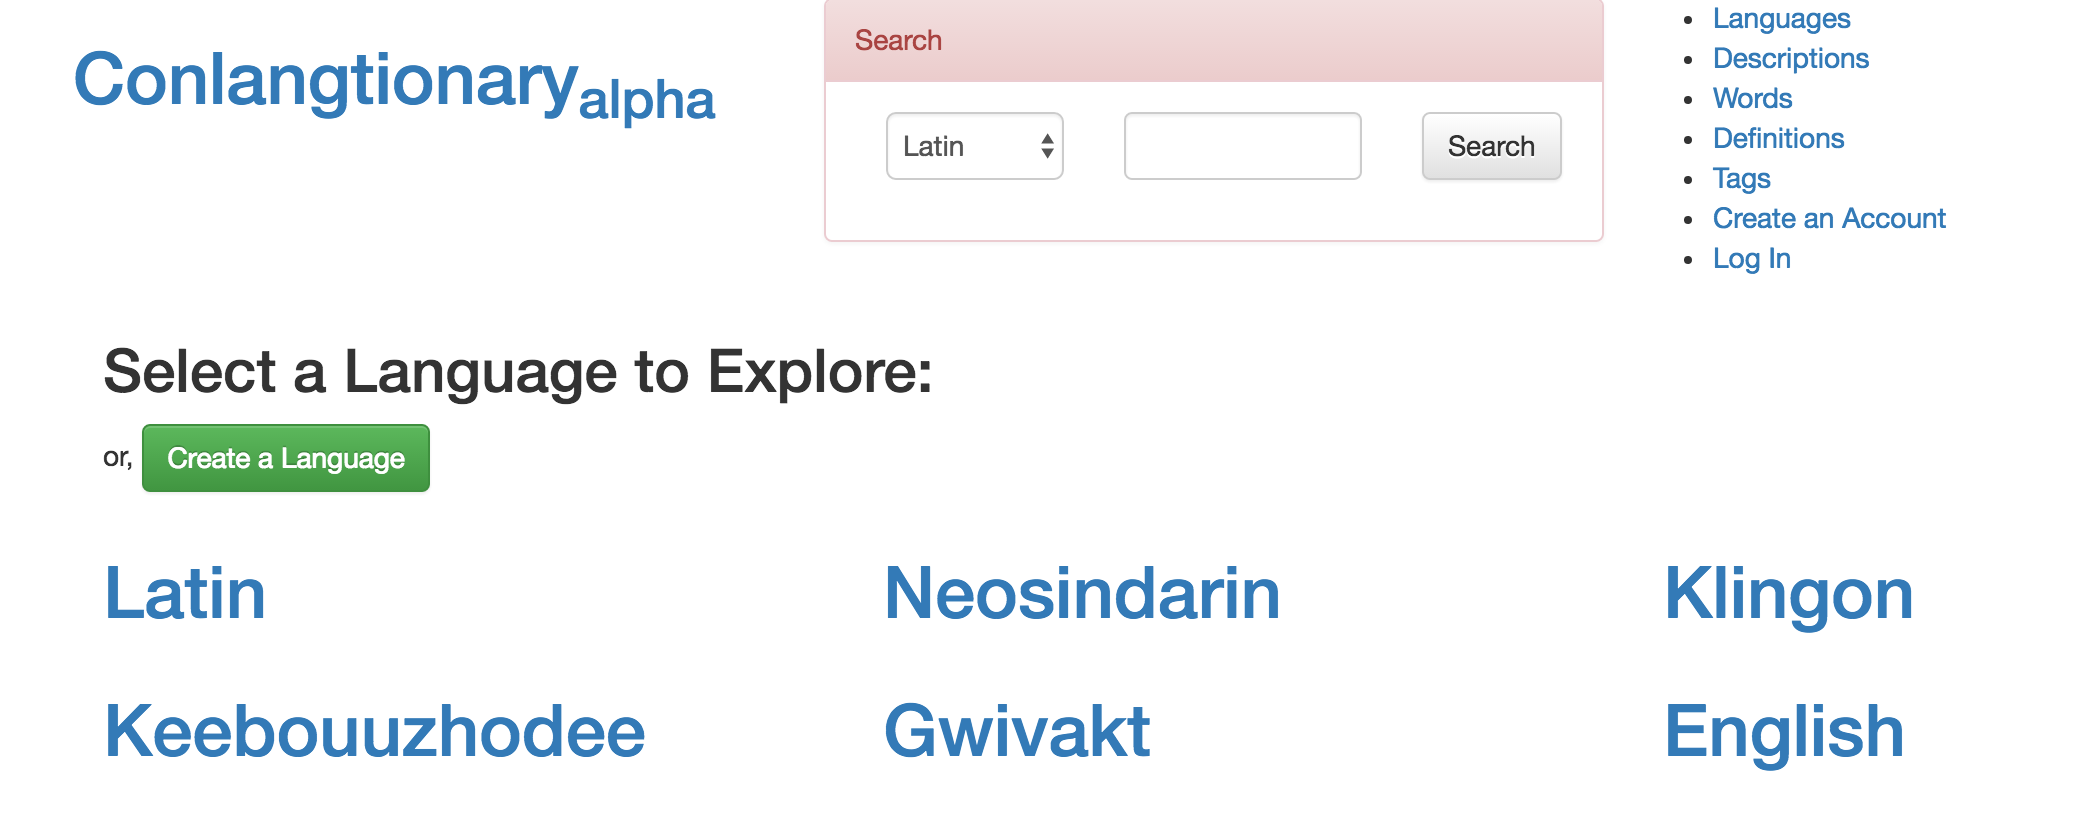
\includegraphics[width=\textwidth]{figures/home-not-logged-in}
\caption{The Conlangtionary Home Page (not logged in).}
\centering
\label{fig:home-not-logged-in}
\end{figure}

\section{Exploring Conlangs}
\label{sec:exploring-conlangs}

To explore a conlang, a user simply needs to click on its name on the home page (the page in Figure \ref{fig:home-not-logged-in}). To return to the home page, a user can just click the site's title (the $Conlangtionary_{alpha}$ in the upper-left of every page).

Every conlang has a page similar to the one depicted in Figure \ref{fig:keebouuzhodee-not-logged-in}. The page is divided into four colored content areas. It is important to note that the color of the area does not have any significance other than distinguishing sections easily. The green section hosts the language's name along with a sentence-length description and any language-level user notes. The yellow area houses all of the language's tags (see Section \ref{subsec:tags}). The blue is the language's description (see Section \ref{subsec:descriptions}). Finally, the red area houses each word with all of that word's definitions listed beneath the word (see Sections \ref{subsec:words} and \ref{subsec:definitions}).

\begin{figure}[!h]
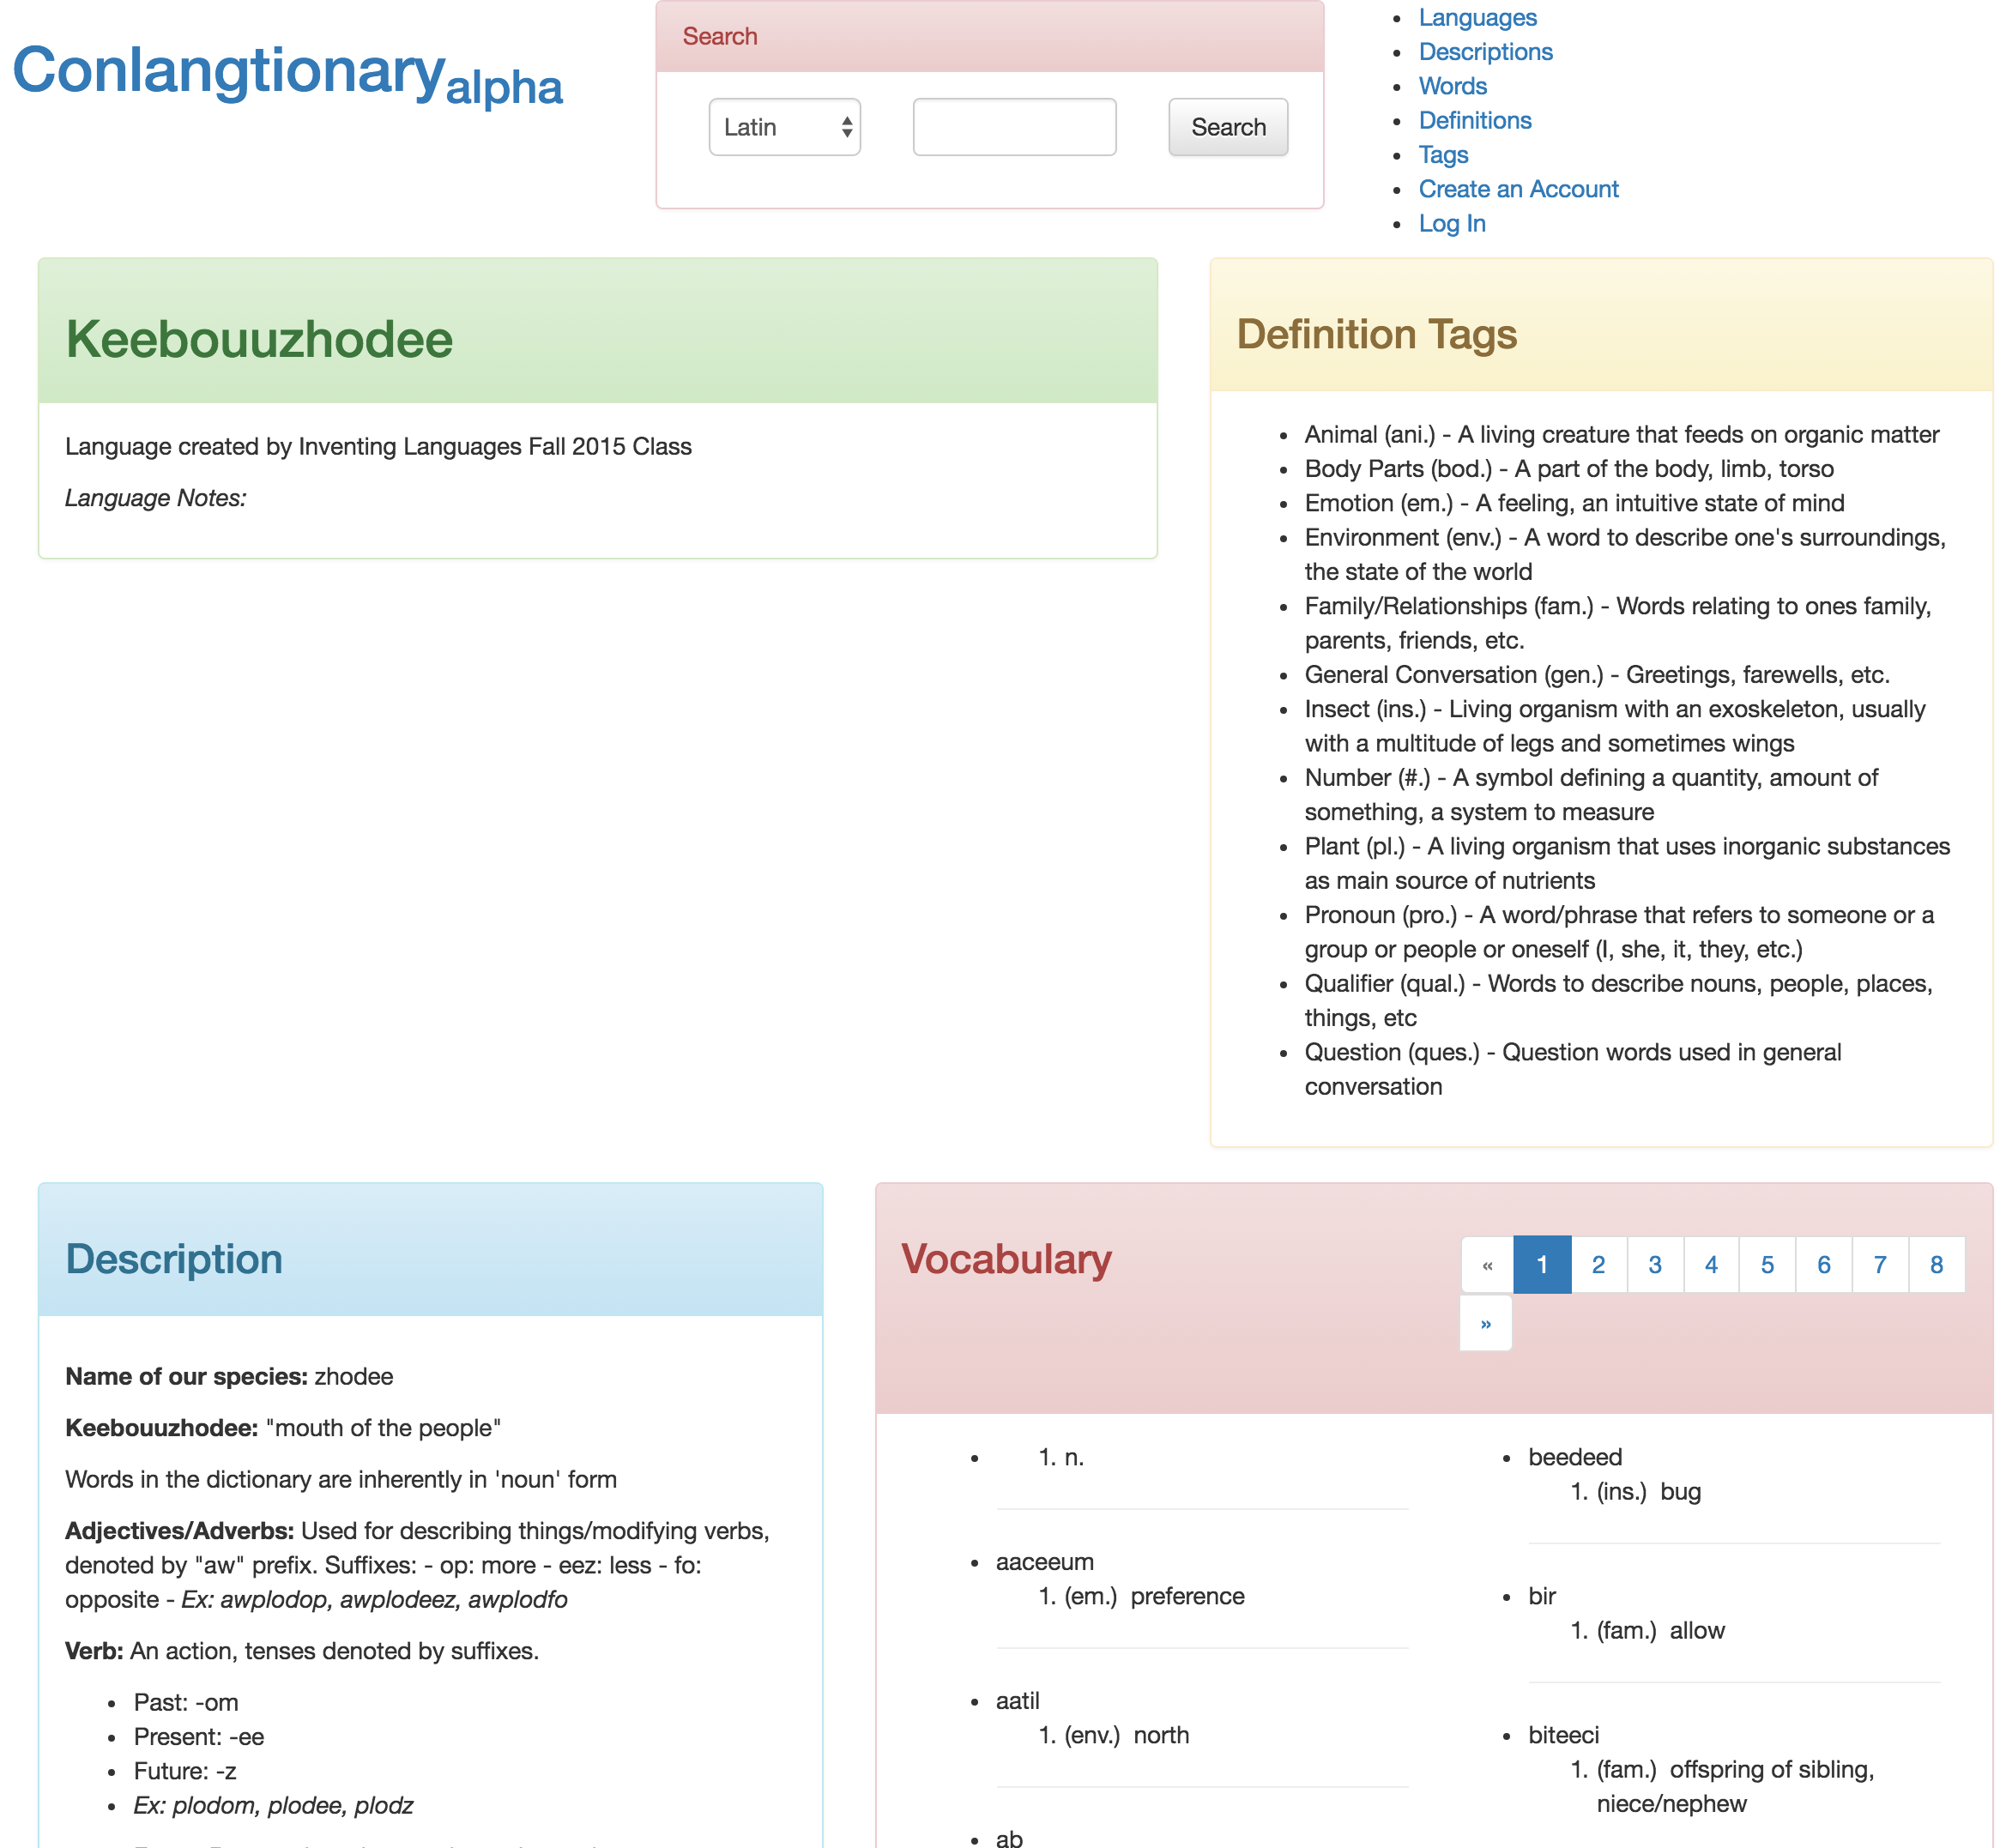
\includegraphics[width=\textwidth]{figures/keebouuzhodee-not-logged-in}
\caption{The Keebouuzhodee Language Page (not logged in).}
\centering
\label{fig:keebouuzhodee-not-logged-in}
\end{figure}

Generally, the description of a language will include a rough summary of the language's grammar and usage. It might also include external links to resources on the language hosted elsewhere. To get a feel for a language, it is best to look at the grammar and usage examples, and then to play around with the vocabulary.

The words in the red area are formatted in deliberate imitation of a dictionary. Each word has definitions listed below it, and those definitions begin with the abbreviations for every tag present on that definition. This means that if a language tags words by part of speech, words will appear with their part of speech before their definition (much like English dictionaries currently do). Every tag shows its abbreviation after its name in the yellow area, so it should be easy for users to figure out what the tags on a definition mean from this page.

\section{Account Registration}
\label{sec:account-registration}

Signing up for Conlangtionary is easy. When a user is not logged in, all they have to do is click on the ``Create an Account" link on the top right of the screen. This takes them to the page depicted in Figure \ref{fig:registration-form}. 

\begin{figure}[!h]
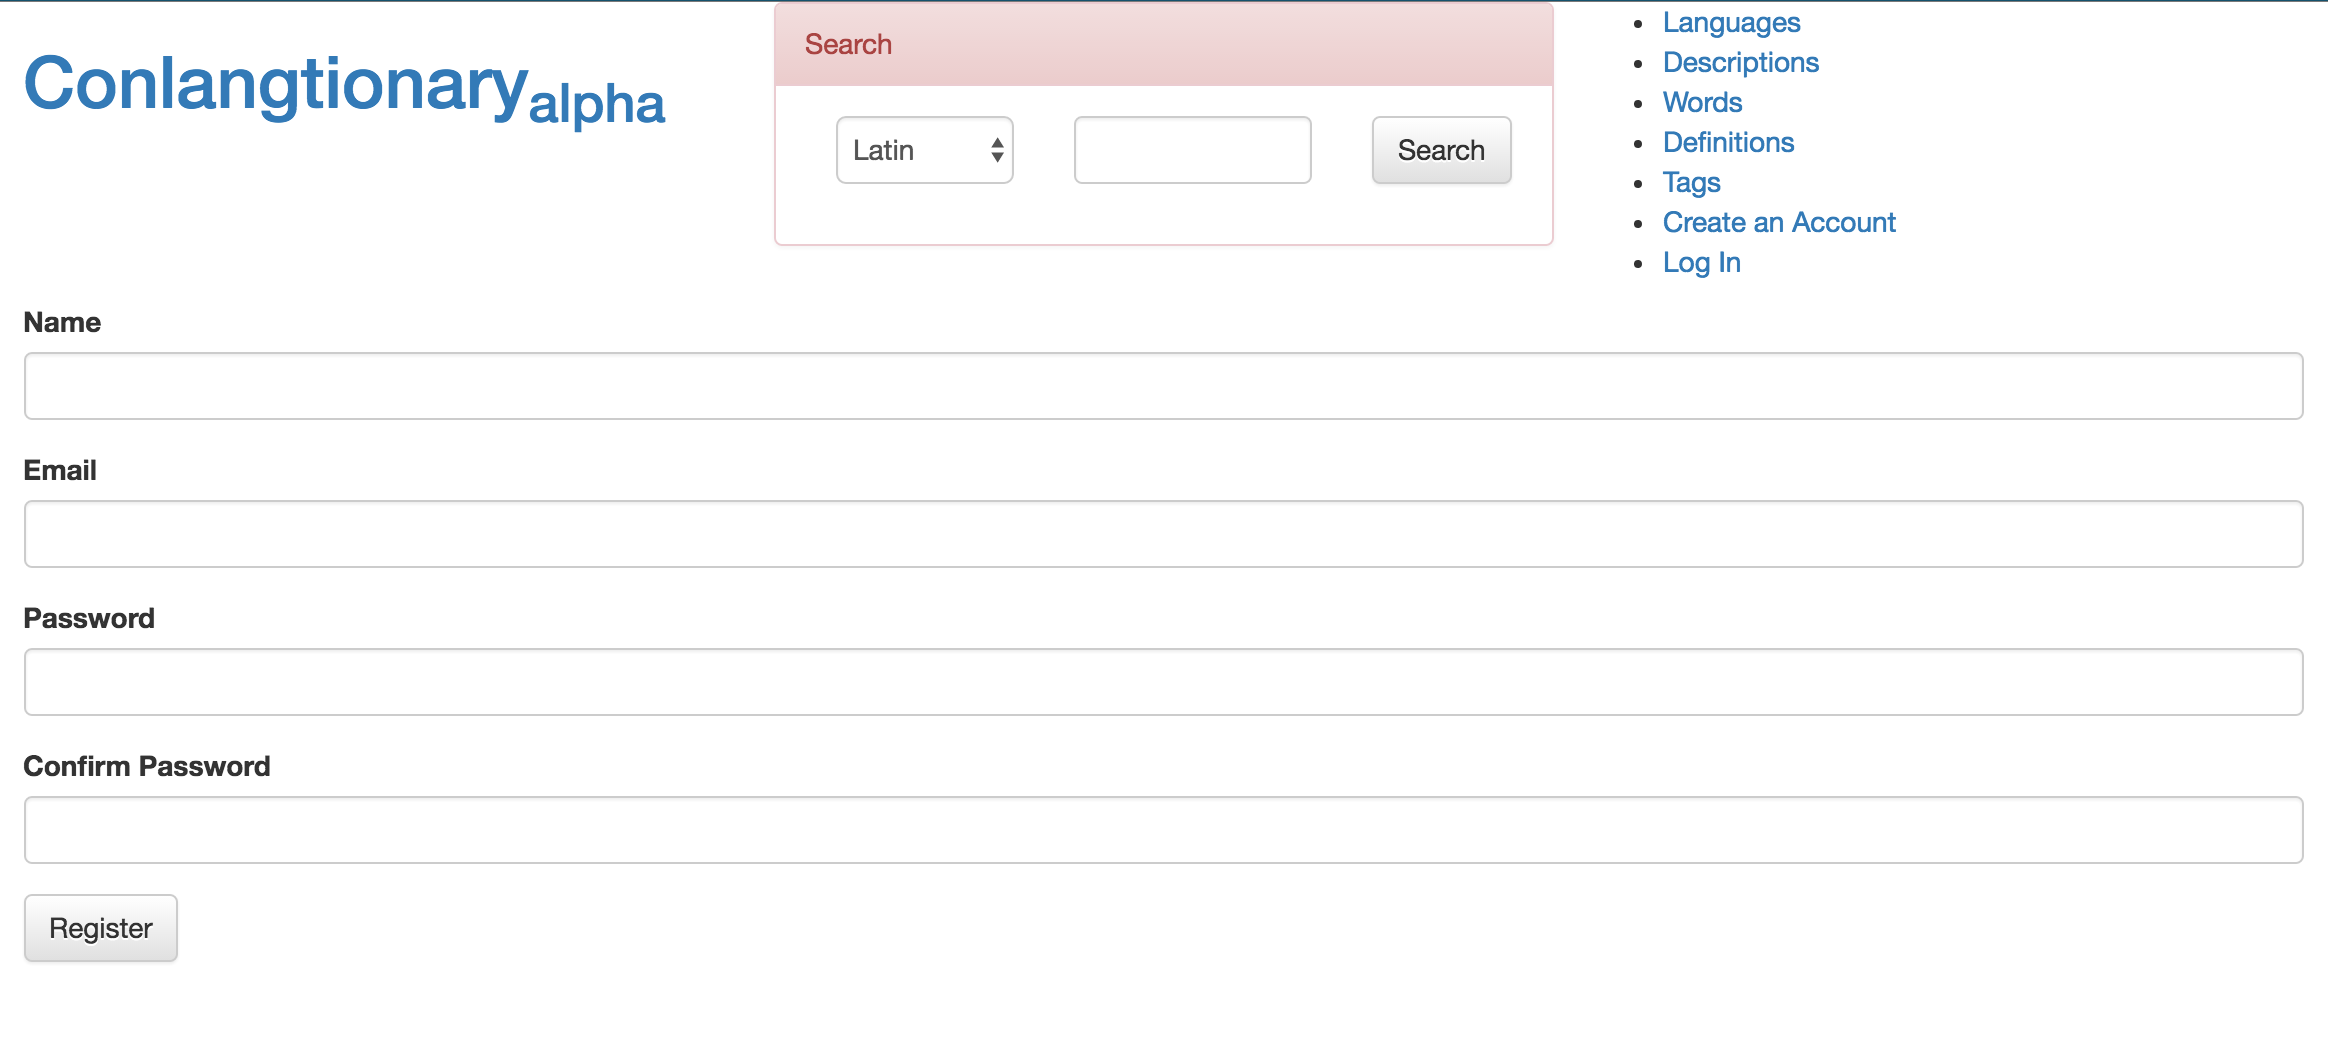
\includegraphics[width=\textwidth]{figures/registration-form}
\caption{The registration form.}
\centering
\label{fig:registration-form}
\end{figure}

Filling out this form creates a user account that can log in with the given username and password combination. There isn't currently any email validation, which does leave the site vulnerable to spam accounts. Once a user has an account, they can just click the ``Log In" link in the future to access the protected features of the site.

\section{Logging In}
\label{sec:logging-in}

\begin{figure}[h]
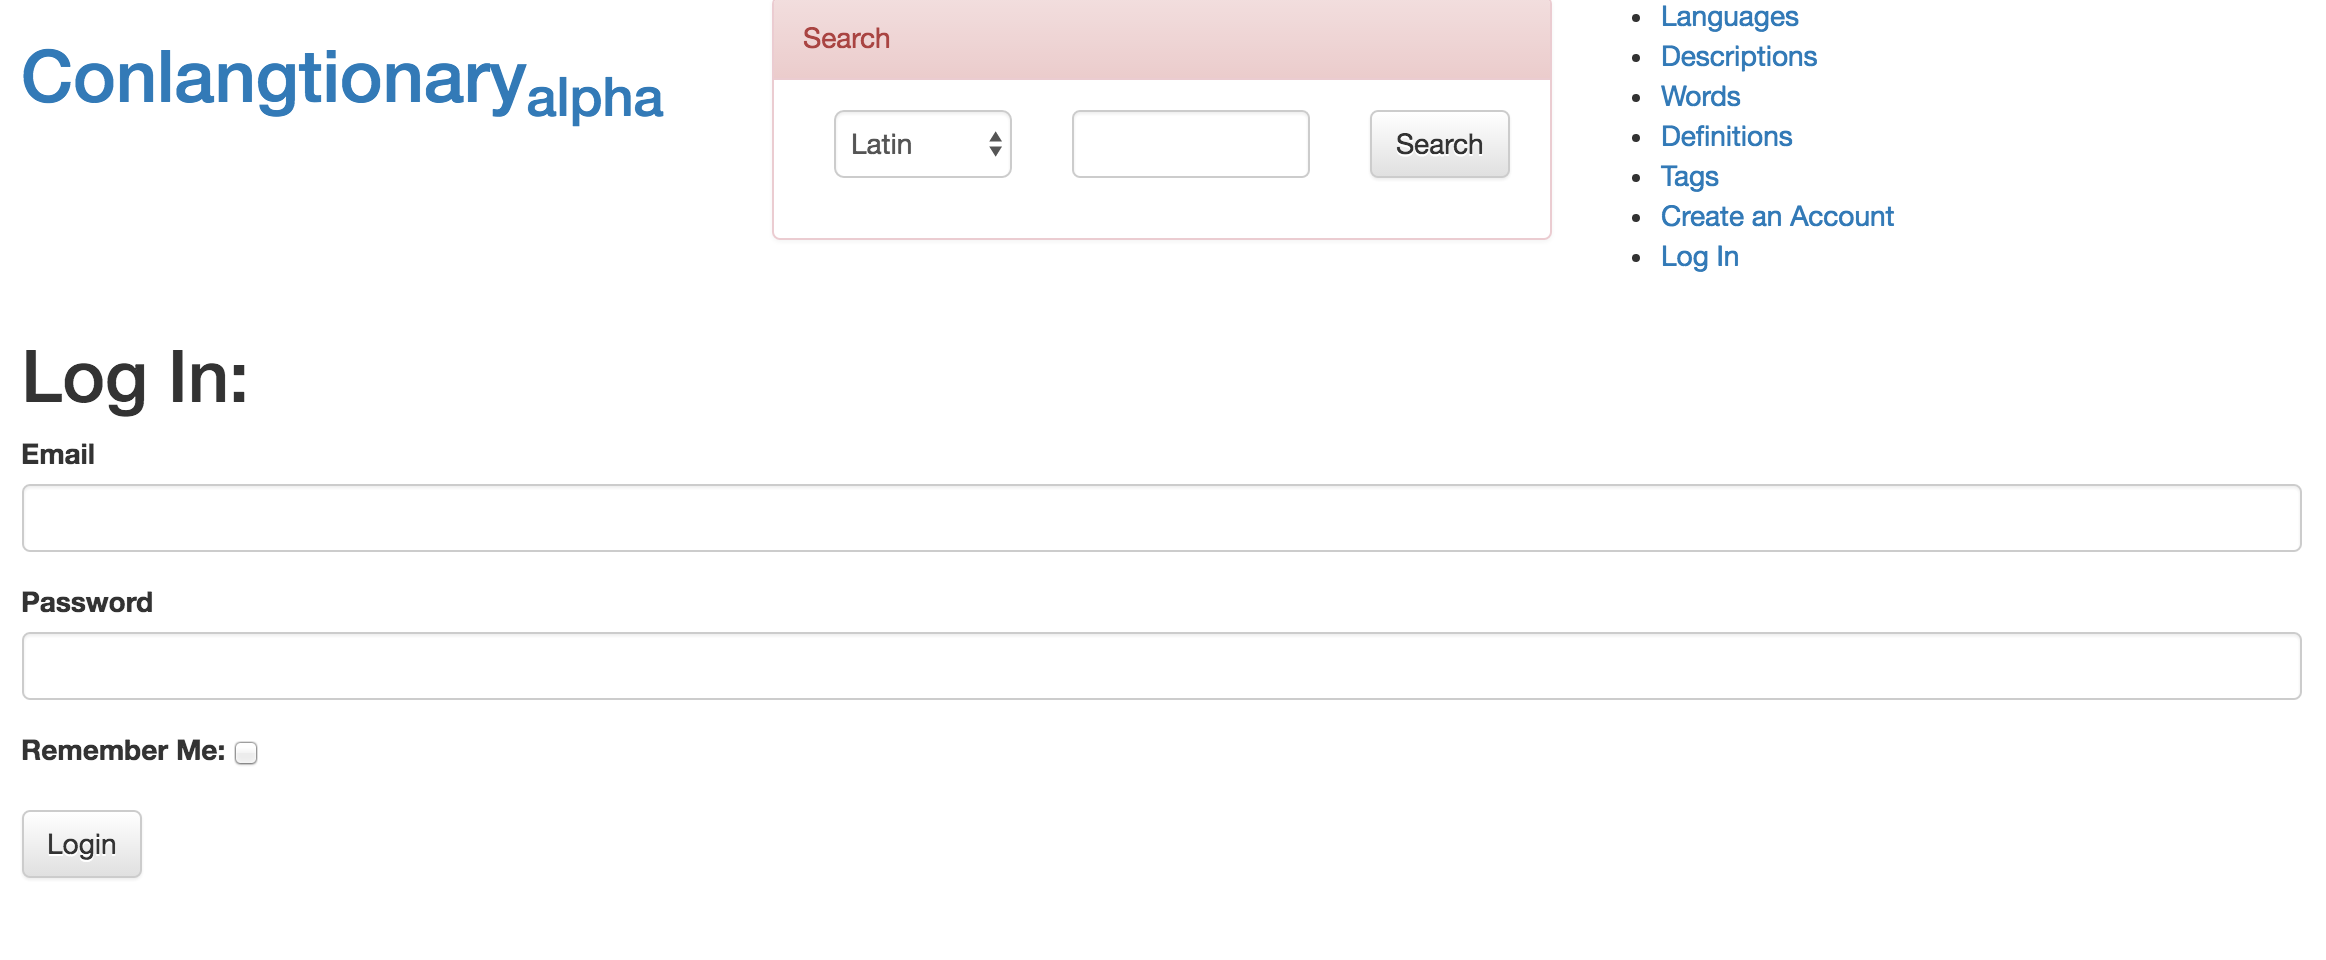
\includegraphics[width=\textwidth]{figures/log-in}
\caption{The login form.}
\centering
\label{fig:log-in}
\end{figure}

Logging into Conlangtionary is simple. Clicking the ``Log In" button in the menu takes a user to the form shown in Figure \ref{fig:log-in}. Filling out a valid email and password combination allows a user into the site.

\section{Creating a Language}
\label{sec:creating-language}

Getting started in Conlangtionary requires a language to work on. There is a button on the home screen labeled ``Create a Language" that begins the process of building a conlang. If a user is not logged in, the button will redirect to a login screen before allowing the user to proceed. The form for creating a language is simple, and can be seen in Figure \ref{fig:create-language}.

\begin{figure}[h]
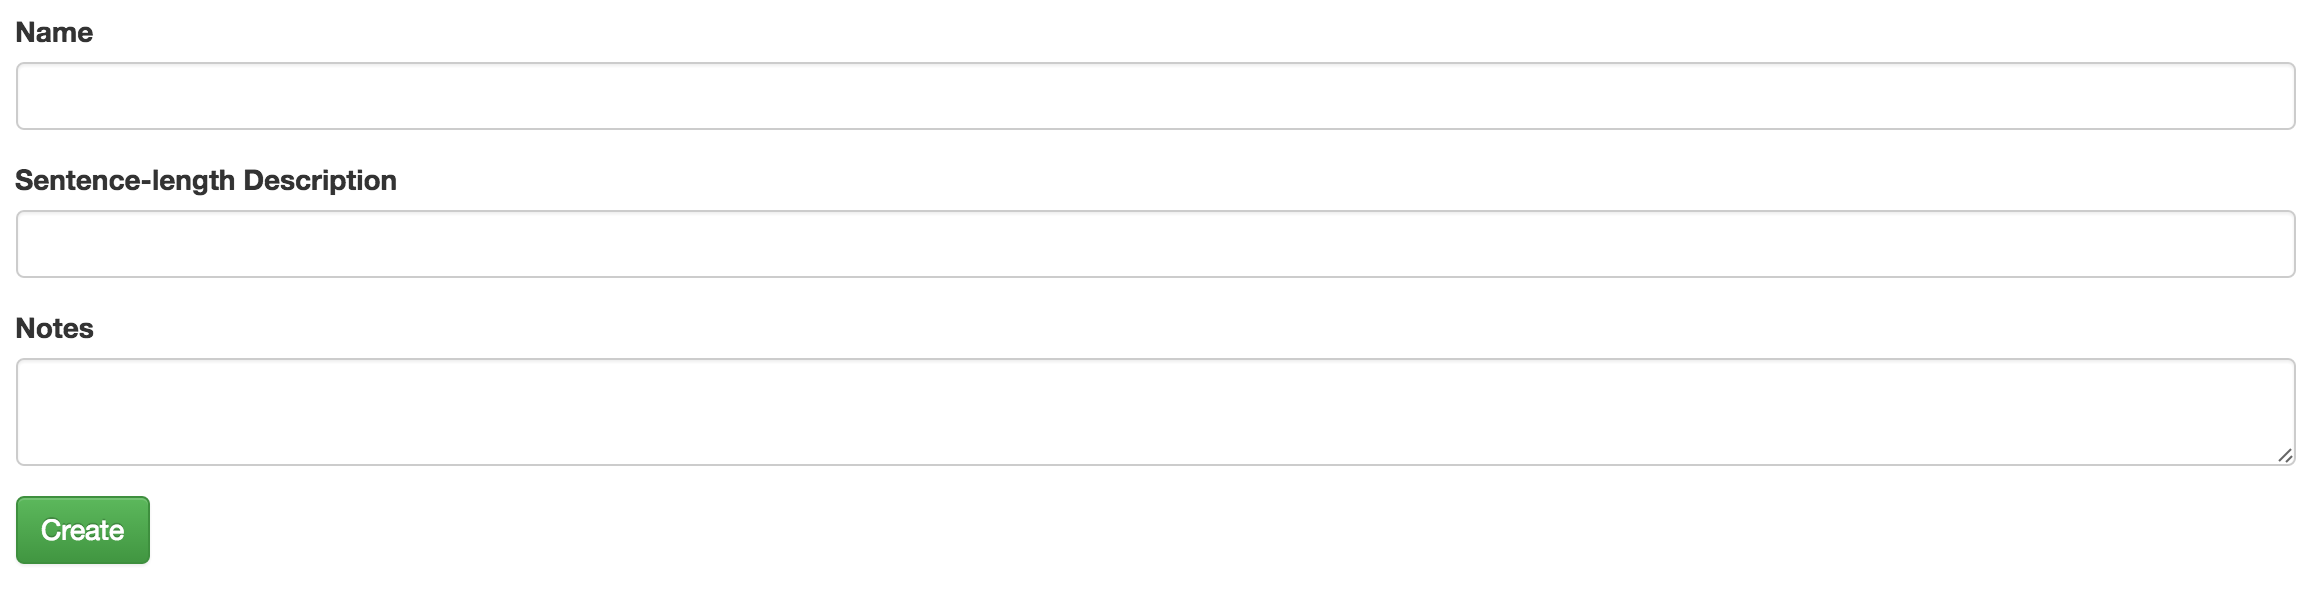
\includegraphics[width=\textwidth]{figures/create-language}
\caption{The language creation form.}
\centering
\label{fig:create-language}
\end{figure}

To create a language, a user must provide some name for that language and a sentence-length description of that language. They can optionally provide notes about that language, though the usage of the notes section varies widely by user.

Once a user submits that form, they are taken to a very empty version of Figure \ref{fig:keebouuzhodee-not-logged-in}, but with controls to manipulate the language. These controls appear because the user is logged in. The empty language with controls can be see in Figure \ref{fig:empty-language-logged-in}.

\begin{figure}[h]
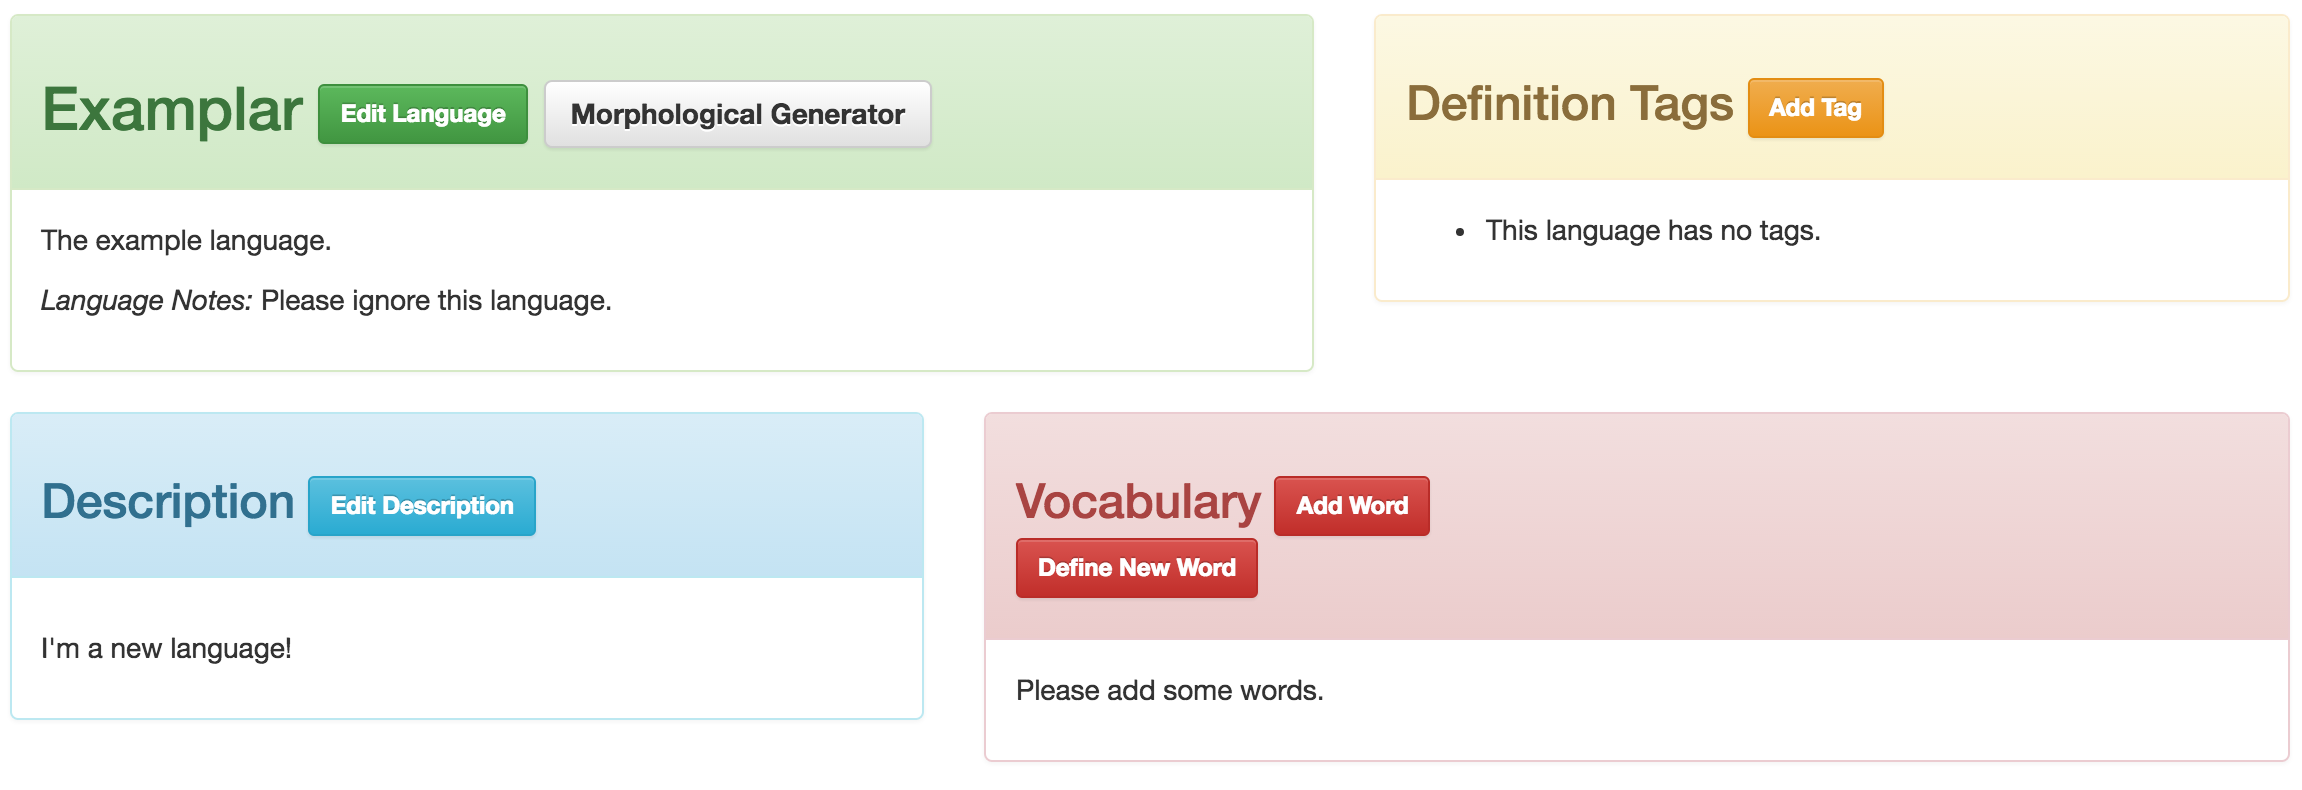
\includegraphics[width=\textwidth]{figures/empty-language-logged-in}
\caption{An empty language.}
\centering
\label{fig:empty-language-logged-in}
\end{figure}

\section{Defining a Word}
\label{sec:define-word}

Languages are built of words, and every word in a language has at least one meaning. To create a word with its first definition, a user can click the red ``Define New Word" button in Figure \ref{fig:empty-language-logged-in}. This will take a user to the form for creating words, which can be seen in Figure \ref{fig:define-word}.

\begin{figure}[h]
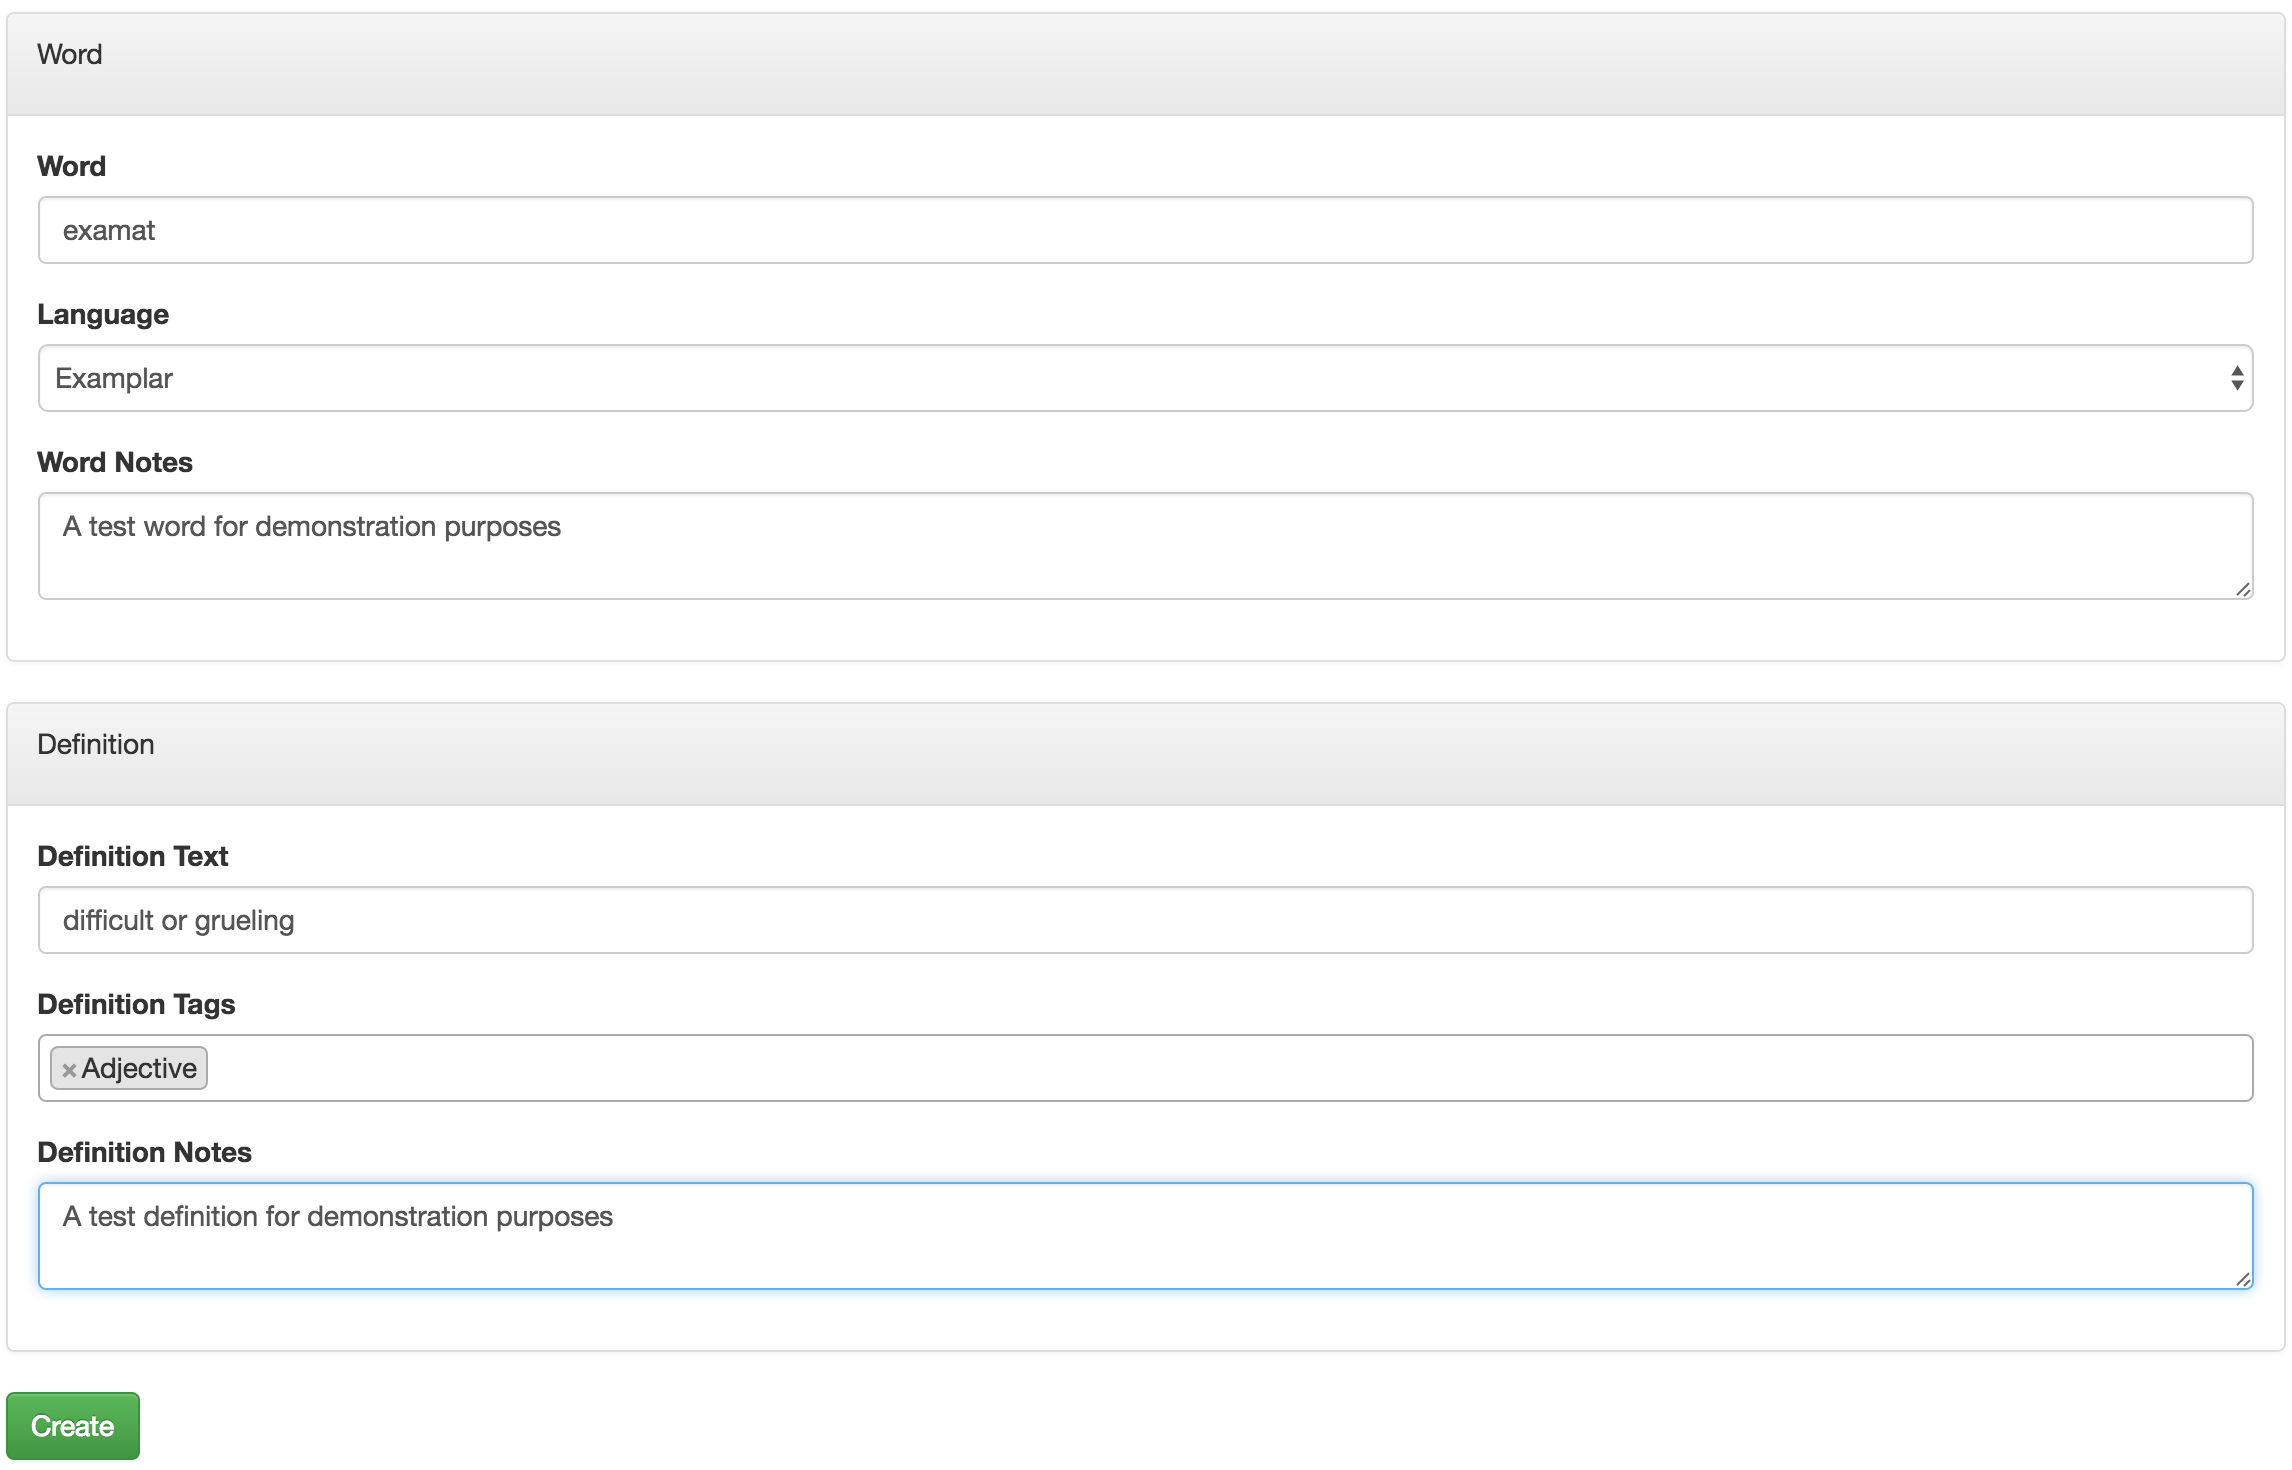
\includegraphics[width=\textwidth]{figures/define-word-filled-in}
\caption{The word definition form.}
\centering
\label{fig:define-word}
\end{figure}

The different form fields are fairly simple. The field labeled ``Word" is looking for the unicode string that this language uses to write down that word. The ``Language" dropdown menu allows a user to change which langauge that they are editing from this form, although this use case has become less and less common as the site has developed. ``Word Notes" can be any text regarding this word. These notes are intended to be a place for conlangers to discuss this word with one another.

The Definition section of the form is used to create this word's first definition. ``Definition Text" is the actual phrase or sentence describing the meaning of the word in a given context. ``Definition Tags" is an input for adding multiple tags to a word. If a user clicks within the ``Definition Tags" form field, it will bring up a dropdown menu of every tag in the language. The user can select as many or as few tags as they wish to. Additionally, typing the name of a new tag and pressing the Enter (or Return) key will create a new Tag in the language that will be attached to this definition. ``Definition Notes" serve the same role as Word Notes, but regarding a specific definition instead of a word.

\begin{figure}[h]
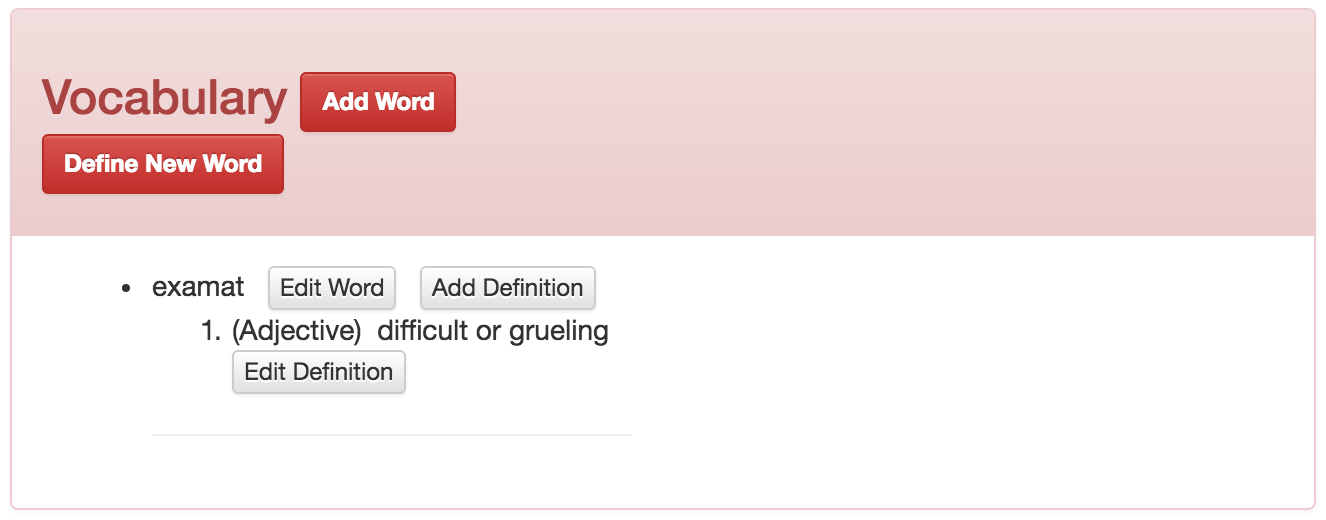
\includegraphics[width=\textwidth]{figures/example-language-one-word-logged-in}
\caption{An example language with its first word and definition.}
\centering
\label{fig:example-language-one-word-logged-in}
\end{figure}

When the user submits this form, they will be returned to the language's page, but it will now contain
their word and definition (see Figure \ref{fig:example-language-one-word-logged-in}).

\section{Creating a Definition}
\label{sec:create-definition}

Once you have a word, adding a definition is straightforward. The ``Add Definition" button in Figure \ref{fig:example-language-one-word-logged-in} takes a user to the definition creation form. The definition creation form has the exact same components as the definition section of Figure \ref{fig:define-word}, and it can be filled out in the same way.

Editing a definition uses this same form. To edit a definition, use the ``Edit Definition" button next to the definition in question in Figure \ref{fig:example-language-one-word-logged-in}.

\section{Creating a Tag}
\label{sec:create-tag}

Creating a tag works much the same way as creating a definition. Using the yellow ``Add Tag" button in Figure \ref{fig:empty-language-logged-in}, a user can access the tag creation form (Figure \ref{fig:create-tag}). 

\begin{figure}[h]
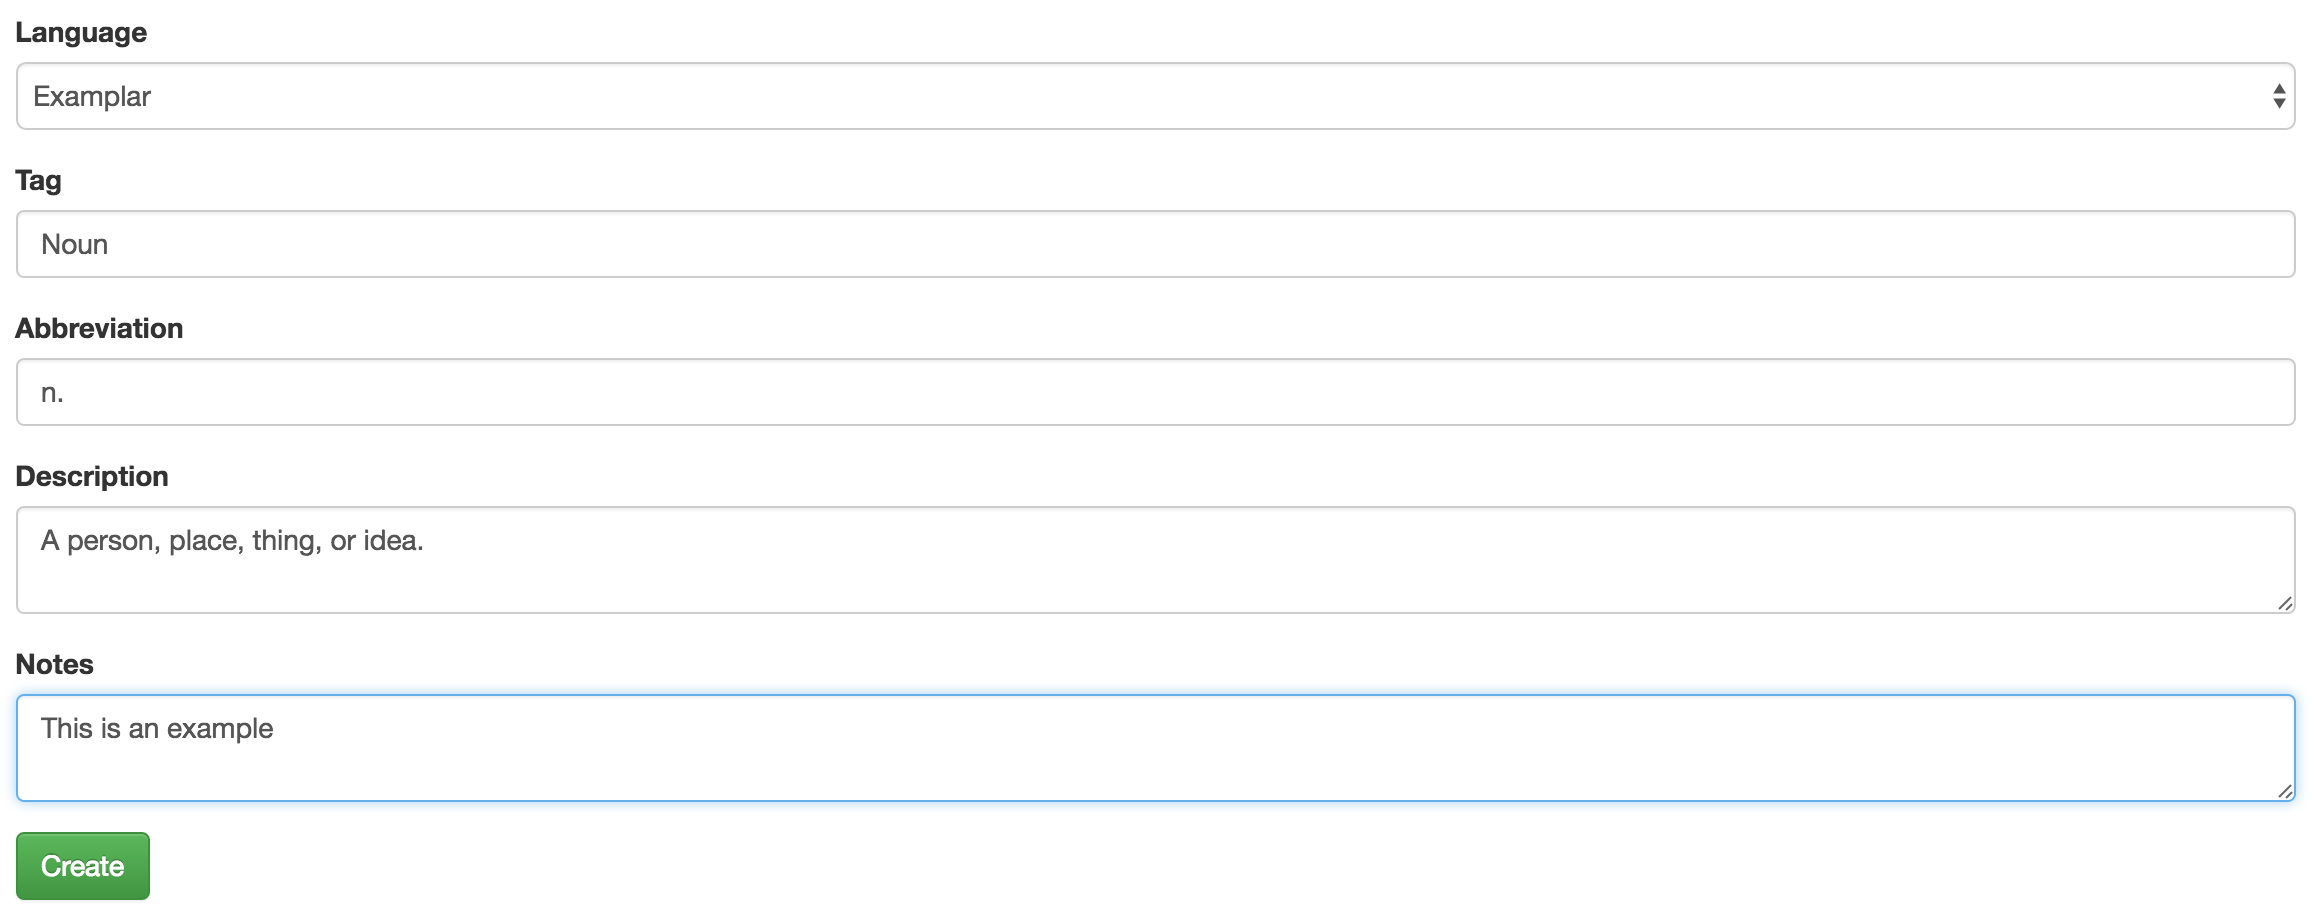
\includegraphics[width=\textwidth]{figures/create-tag}
\caption{The tag creation form.}
\centering
\label{fig:create-tag}
\end{figure}

The tag needs a name. Since tags can be used to encode any kind of information about a definition, it is difficult to suggest what to use. If a user is encoding parts of speech, the name of that part of speech will suffice. 

Tags also ask for an abbreviation. This will be displayed before the definition text of any definition with that tag. For parts of speech, this makes it very easy to display (n.) before nouns and so forth.

The tag description is a text description of what it means for a word to bear that tag. For parts of speech this can be a description of the role of that part of speech, but for other kinds of tag this can become quite complex. For instance, if a user were to tag by verb conjugation type, the description would need to explain how that type conjugates, or at least the difference between words in that class of conjugation and other words in the language.

As with every data entity in Conlangtionary, tags can also have notes, which ought to be used for internal reference and collaboration on the part of conlangers working with the language.

\section{Editing the Description}
\label{sec:edit-description}

The language description is simply a text area that supports the Markdown text format \cite{Markdown}. Users can write any content related to the language that they desire. Because it uses Markdown, users can even provide links to external resources about their languages if they desire.

The form looks like Figure \ref{fig:edit-description}, and it provides a link to resources on Markdown for users who might be unfamiliar with the format.

\begin{figure}[h]
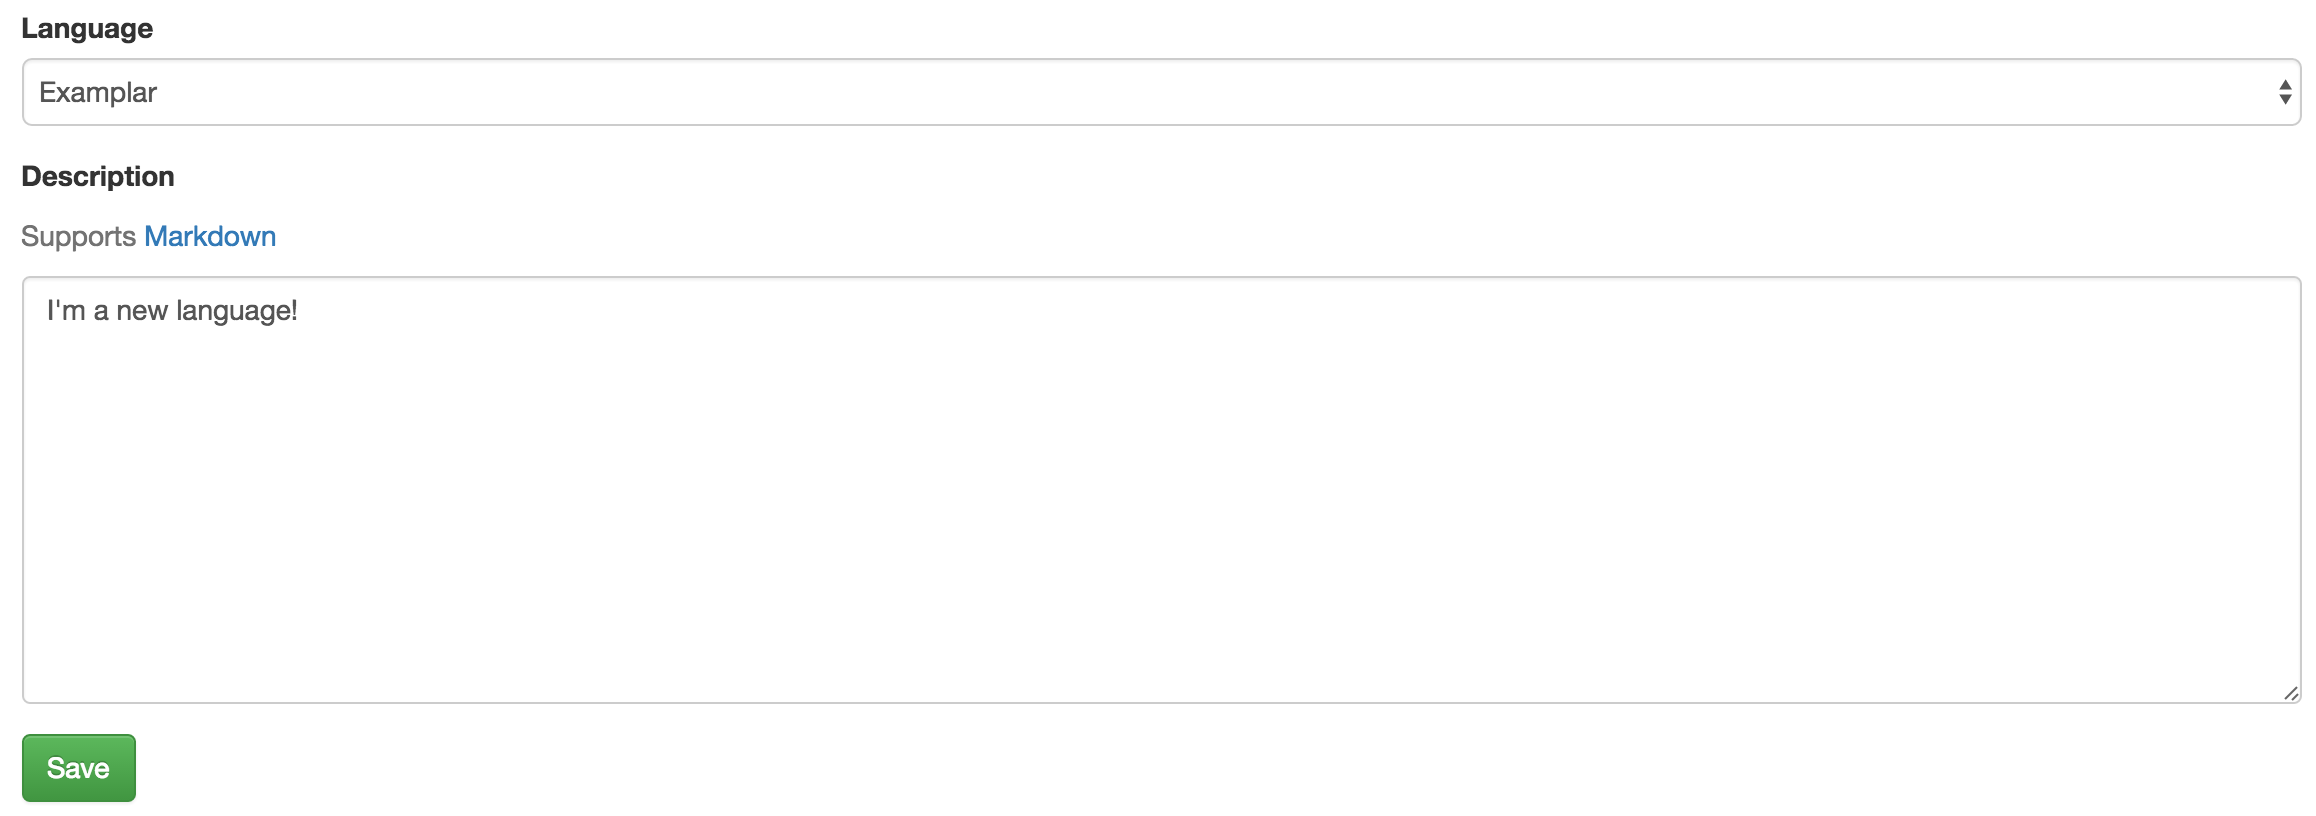
\includegraphics[width=\textwidth]{figures/edit-description}
\caption{The description editing form.}
\centering
\label{fig:edit-description}
\end{figure}

\section{Using the Morphological Generator}
\label{sec:using-morph-gen}

The Morphological Generator is the real power tool at the heart of Conlangtionary. Without it, Conlangtionary as a platform is just a descriptive tool. With it, Conlangtionary becomes a generative tool in its own right.

Morphological Generation is all about transforming a word from one form to another. To start with, Conlangtionary assumes that the word (or, more accurately, the word's definition) is tagged with all of the necessary information to distinguish between words that should be transformed and words that should not be affected. If definitions are not tagged with sufficient granularity, the generator will be useless for that language.

For example, if a user has tagged all of the Adjectives in a language simply as Adjectives, they could easily transform adjectives into a noun form \textit{if} all adjectives morph into nouns following a single, consistent rule. For the sake of a simple example, assume that the language in question is called SIMPLE and has the rule that any adjective can be made into a noun by adding the suffix ``ack." To turn the made-up SIMPLE adjective ``yasson" into a noun, one simply makes it ``yassonack." To perform this change, a user can simply tell Conlangtionary to take all definitions in SIMPLE with the tag ``Adjective" and add ``-ack" to the end of their word forms to create new words with the same definition as the Adjectives but tagged as ``Noun". If that rule has exceptions, then the generator cannot be applied unless all of the words that follow the rule share an additional tag that the words that do not follow the rule lack. If all of the adjectives that follow the rule share the tag ``Regularly-Nominalized," the generator can still perform the transformation. The only difference would be that it must select definitions bearing both the ``Adjective" tag and the ``Regularly-Nominalized" tag.

To specify this transformation through the user interface, a user must click the gray ``Morphological Generator" button seen in Figure \ref{fig:empty-language-logged-in}. This will bring a user to the page shown in Figure \ref{fig:morphological-generator}.

\begin{figure}[h]
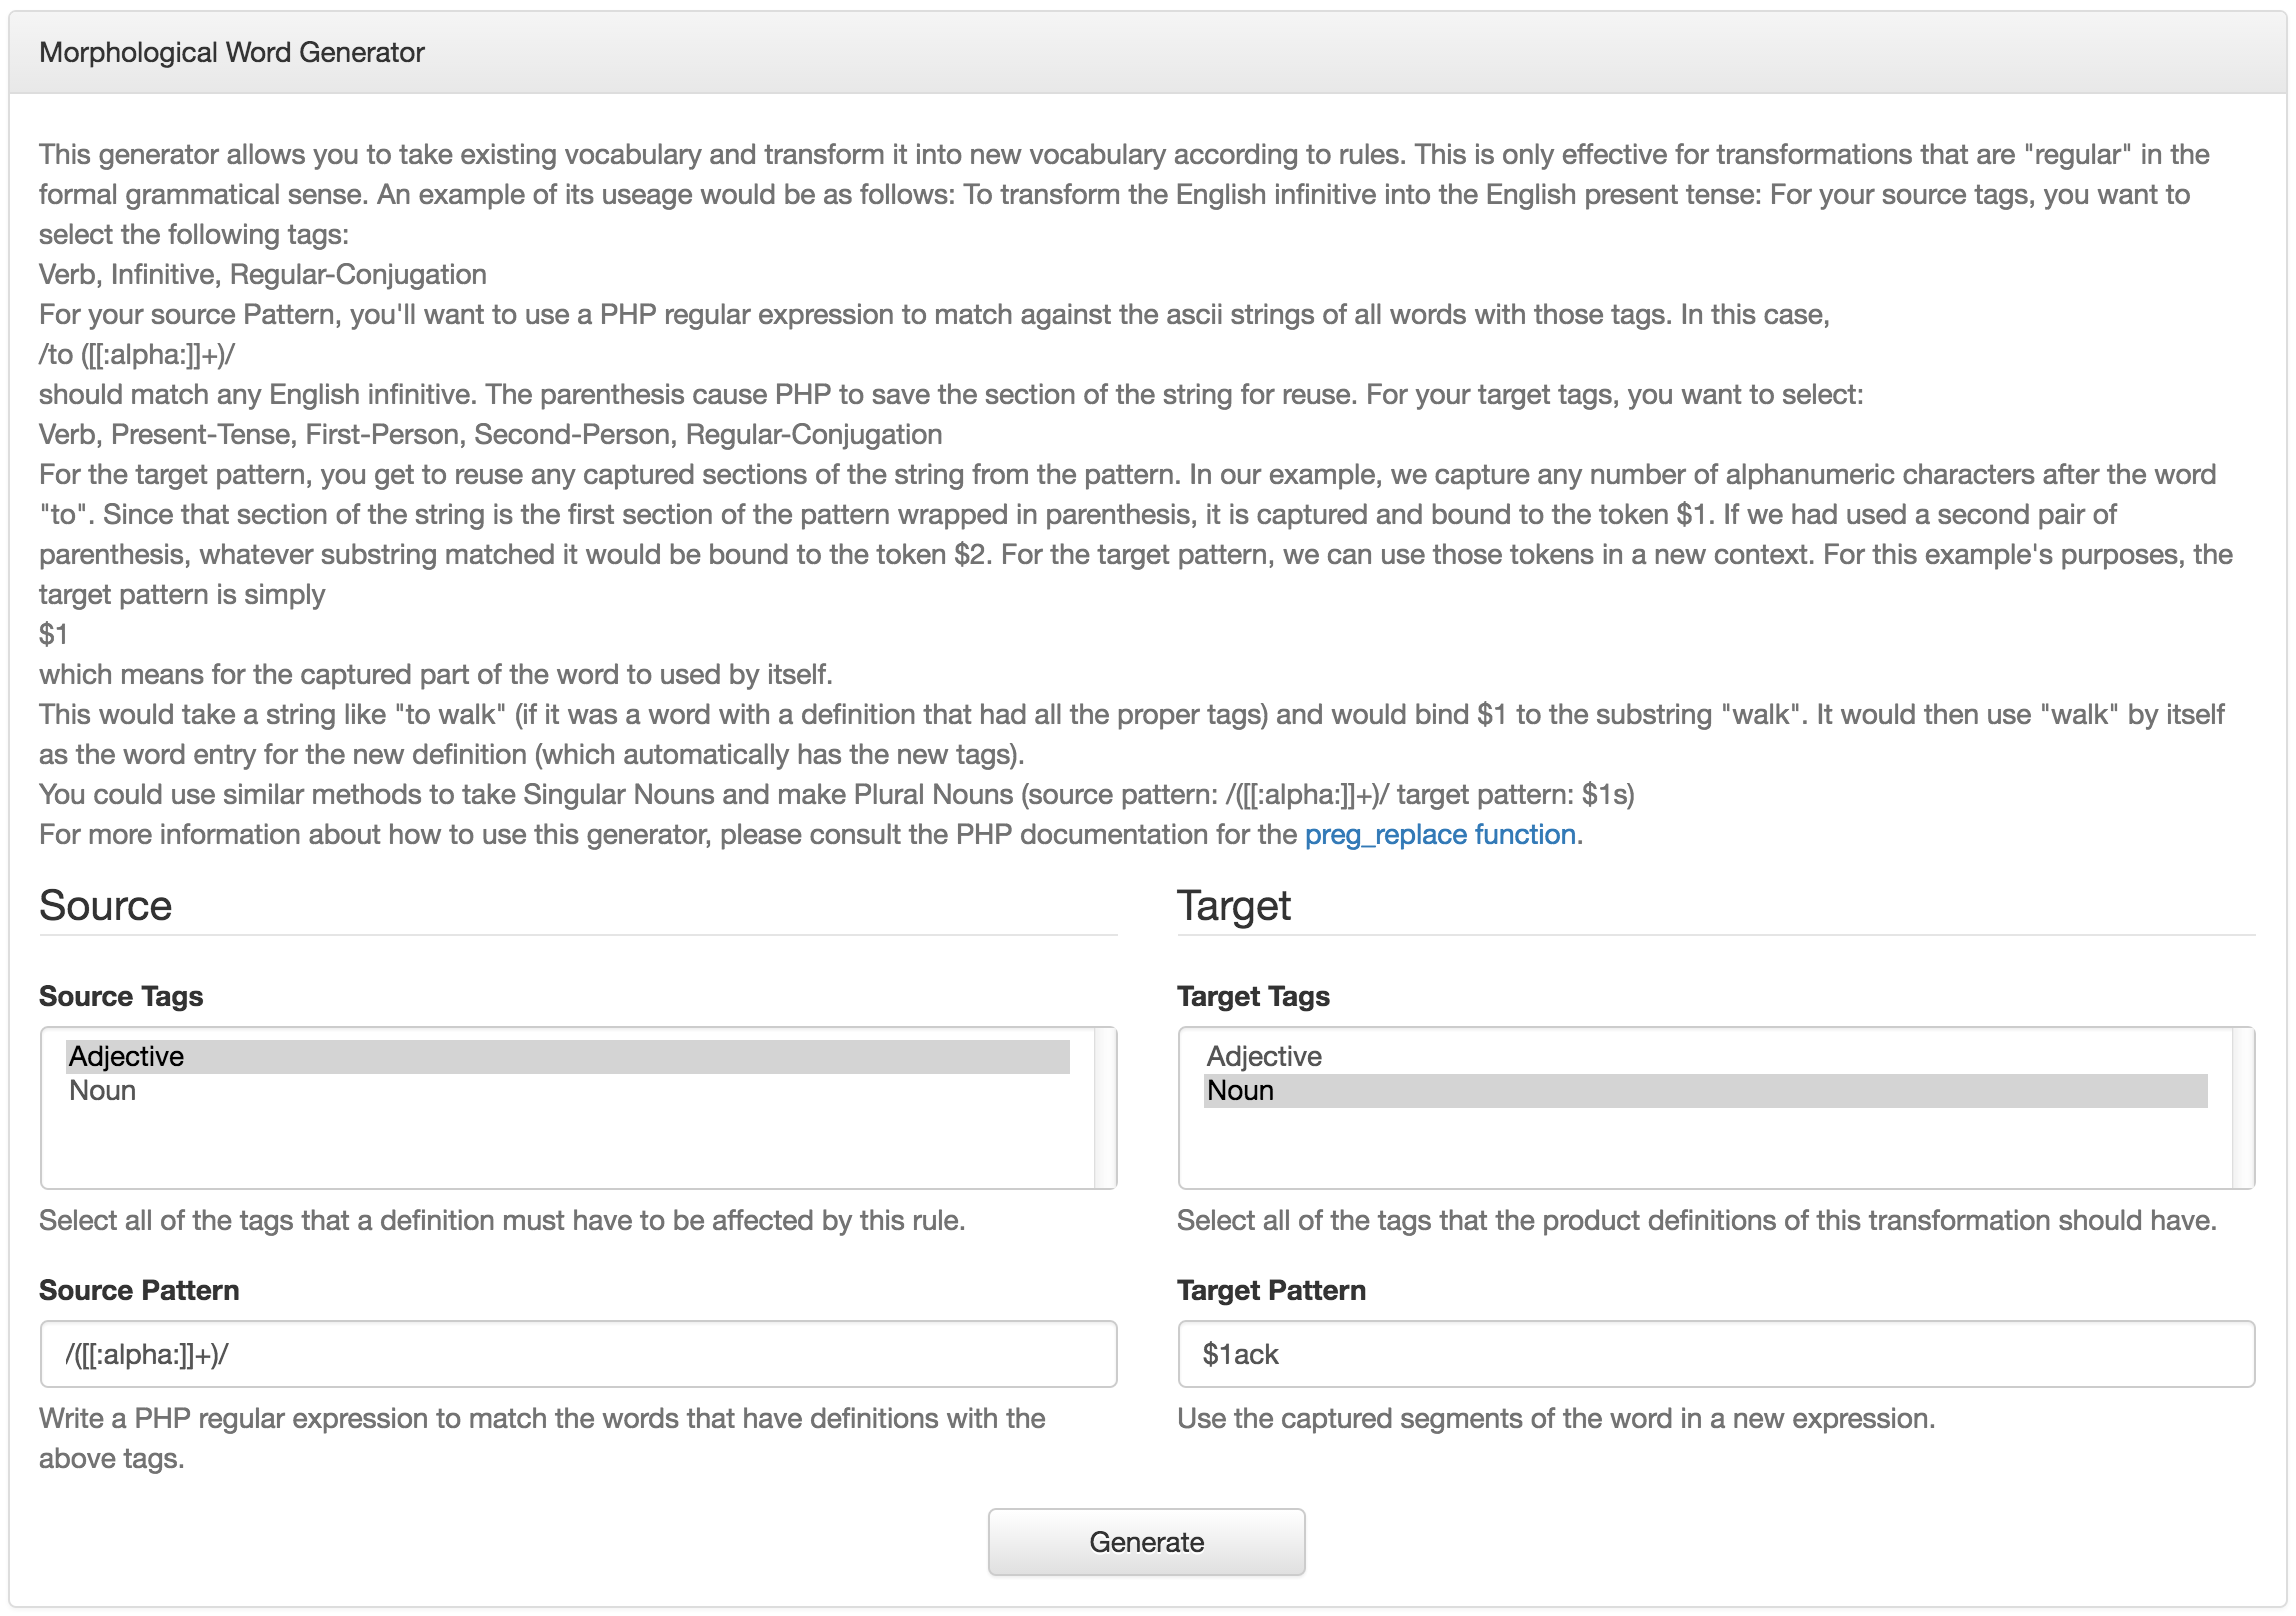
\includegraphics[width=\textwidth]{figures/morphological-generator-filled-in}
\caption{The morphological generator.}
\centering
\label{fig:morphological-generator}
\end{figure}

There is an explanation of the use of the generator on the page, but another is included here for the sake of completeness.

First, a user should select the tags that they want to operate on from the ``Source Tags" multi-select form element on the left. To select more than one, hold down the control key when clicking. Once the source tags have been chosen, the user should insert a PHP regular expression into the ``Source Pattern" input. This pattern is used to recognize and capture parts of the words that are needed in the result of the transformation. In the case of the above example, the user would select Adjective as a source tag and would use the pattern \url{/^([[:alpha:]]+)$/} to capture the entire word as an adjective.

After configuring the source information, the user follows a similar procedure to specify the output of the transformation. ``Target Tags" are the tags that the definitions created by the generator will bear, and ``Target Pattern" specifies the structure of the words that those definitions will define. To continue with the same example, the target tag would be ``Noun" and the target pattern would be \url{$1ack}. The ``\$1" is replaced with the first item from the source pattern that was surrounded by parenthesis. Since the source pattern surrounds the whole word with parenthesis, the target pattern will append ``ack" to the source words and define them tagged as nouns instead of adjectives. The definitions may need to be rephrased to reflect that the words have changed parts of speech, but such changes are too subtle to be automated.

Once a user clicks ``Generate," Conlangtionary will transform all matching words and insert them with the same definitions text that they had before. The difference will be that the definitions will bear different tags. While this may not seem exceedingly useful in the above instance because the user might need to rewrite dozens of definitions, it can very easily be used to generate alternative conjugations of a verb or declensions of a noun without needing to change any definition text.
        \chapter{Future Research}
\label{chap:future}

Conlangtionary is a prototype system. Though it does surpass a platform like a wiki for representing a language, the awkward design of its user interface and access control system hold it back from being an immediate replacement for current online conlanging platforms. At its core, though, Conlangtionary does have a solid model for representing spoken languages. To make it ready for the conlanging community at large, it needs a number of substantial refactors. This chapter details each major area that could benefit from change.

\section{Access Control Refactor}
\label{sec:refactor-access}

As discussed in Section \ref{sec:access-control}, Conlangtionary implements a very simple policy for which users can perform which tasks. Admins can do all actions to all content, authenticated users can do anything but delete content, and nonauthenticated users can only read content. While this simplicity made Conlangtionary's code simpler, it made users unable to destroy erroneous data. While users still had the option to edit an incorrect word or definition to make it valid, it would be simpler to just allow them to delete the content. A more developed system could be implemented as follows:

Content can be marked as public or private. Content belongs to a single ``creator" user, a single ``owner" user, and many (or only one) ``contributor" users. The creator of a piece of content controls who else can own it. This includes removing themself from the owners of the content, after which time they lose the ability to modify who owns the content. Any owner of a piece of content can edit or delete it.

\section{Tag Refactor}
\label{sec:refactor-tag}

Tags are a great, flexible, expressive way to cluster vocabulary into arbitrary categories with user-defined meaning, but the current implementation has one flaw: tags cannot form internal hierarchies. Currently, if your language operated with multiple types of pronoun, you would need a tag for each type of pronoun. If your language also operated on pronouns as a whole, each definition that defined a pronoun would need both the ``pronoun" tag and the ``demonstrative pronoun" tag (for example). 

At first glance, this system seems fine, and it is adequate to group words. However, the experience of adding multiple necessarily-related tags to a word rapidly becomes tedious. If a user has already placed a definition into a subcategory of ``pronoun" (by tagging it as a ``demonstrative pronoun"), why should they need to tag it as a ``pronoun" as well?

This problem can easily be solved by allowing tags to form a tree, much like biological taxonomy. Give each tag a reference to another ``parent" tag at the database level. If a word is tagged, it inherits all of the parent tags of its tags. This would require relatively little work on the database side of the application, but significant refactoring of the User Interface and of the logic that creates definitions and tags.

\section{Definition Augmentation}
\label{sec:refactor-definitions}

Currently, definitions are some text that defines the word, a set of tags that apply to that definition, and some notes about that definition that can be used for essentially any purpose. These features suffice, but there are two major areas in which definitions can be improved.

Firstly, definitions could include a field for a pronunciation guide. This string could be written in the International Phonetic Alphabet or in phonetic English; the only important thing is that it helps the user discern the correct way to pronounce the word \cite{IPA}. This refactor requires small changes to the database, creation logic, and user interface, but does not introduce any serious overhead to the system.

The second augmentation is related. Conlangtionary could store a pronunciation audio clip so that users could record a correct pronunciation of a term when they defined it. This method is less ambiguous (especially if the pronunciation string is in IPA, which few laypeople know), but requires more systemic changes to the platform. Storing audio clips requires significantly more storage space than storing text, and playing them through the user interface would mean adding controls and appropriate libraries of Javascript to handle audio playback.

\section{Description Removal}
\label{sec:refactor-description}

Descriptions in Conlangtionary were intended to provide a place for conlangers to add any miscellanous information about their language that didn't easily translate into the structure of a Conlangtionary language. Information such as grammatical usage, example texts, and the history of the people or culture to whom the conlang belongs. While this is a necessary component of a conlang (cultural context), structuring it as a single blob of text was a mistake. This design forces a conlanger to maintain an enormous single document containing essentially all prose information about their language. They also are forced to do that maintenance through Conlangtionary's markdown editor which, although useful, is not full-featured enough to make for a pleasant editing experience.

As an alternative to this single-blob-of-text approach, a future version of Conlangtionary ought to allow multiple pages of reference material to be attached to a language. On the database level, this is simply a refactor from a one-to-one to a one-to-many relationship between languages and descriptions, though the data that descriptions need to store would change to include titles and perhaps other resources like embedded images.

This would allow the user to define a reference manual for grammar separately from reference material about a conlang's culture. These separate documents of information could also be included as chapters in the proposed Dictionary View (see Section \ref{sec:refactor-dictionary}).

\section{Dictionary View}
\label{sec:refactor-dictionary}

As Conlangtionary's name suggests, it is a dictionary for conlangs. It stores information about the words that make up a conlang and their meanings. In several places, user-interface decisions were influenced by conventions from physical dictionaries (the formatting of definitions on a language view, for instance), but Conlangtionary itself doesn't currently generate an actual dictionary document for a given conlang. The system has all of the requisite data. Generating a PDF of the language with all of the reference materials at the beginning followed by an alphabetical listing of all of the language's words is a decent-sized addition to the code, but a very powerful one.

To do this, Conlangtionary would need to incorporate a package for writing PDF files and then define the structure that the dictionary would take as a view.

\section{User Interface}
\label{sec:refactor-ui}

Conlangtionary's user interface is usable, and that is all. It doesn't look good, nor is it intuitive. It was designed by a programmer, and as such, is only intuitive to its designer. This paper does not set out to propose an alternative user interface, but merely to acknowledge the need. This goal would be easier to accomplish in conjunction with Section \ref{sec:refactor-api}.

\section{Application Programmer Interface}
\label{sec:refactor-api}

This is the most ambitious of the proposed refactors: rewrite essentially the entire application around a more modern paradigm. When Conlangtionary was initially designed, Laravel was chosen as the framework because it was familiar to the designer \cite{Laravel}. While Laravel has many features that are modern, Conlangtionary is written in such a way that it handles both the logic that processes data and the logic that renders that data to the user. The two cannot be easily separated. Modern web development separates these two sets of logic into the front-end (display the data) and back-end (store, manipulate, and retrieve the data). This abstraction allows the two sides of an application to be developed separately.

If this change were adopted, some of the existing Laravel code could be reused. Namely, the Controller logic that creates, reads, updates, and deletes Models would only need to be altered to return data instead of HTML. The front end would need to be completely rewritten. Technologies like Backbone and React would be good choices for making the front end a powerful application.

Ideally, the front end of the site could be written as a single page that allows users to act on each part of a language (definitions, words, descriptive text, and even grammatical rules) without navigating away from that page. This would be significantly more efficient in terms of the number of clicks that it takes for a user to perform a given action on a language.

\section{Language Assumptions}
\label{sec:refactor-language-assumption}

In a platform designed to represent languages of unlimited variety, the fact that the web application itself is fundamentally English-oriented is nearly inexcusable. Technically, since Conlangtionary supports Unicode, a user can define words in any left-to-right language within the Unicode character scheme, but this doesn't change the text on the controls of the site or the paragraphs of explanatory text on the Morphological Generator. This makes the application considerably less useful for non-English-speaking users.

Additionally, the structure of a Definition within Conlangtionary assumes that the user is defining the term in the Conlang in a single other language. This prevents any possiblility of defining a conlang on the site in terms of another conlang. A better system would define definitions as a transformation of a term from a target language into a destination language (which could be itself). For instance, defining the English term ``walk" as ``to move with your legs at a speed that is slower than running" transforms an English term into alternative English terms, but defining Spanish ``caminar" as English ``to walk" is a transformation between languages \cite{Merriam-Webster:walk}. Both of these transformations are expressible in terms of a target and destination (alternatively, they could be called source and destination languages). Such a structure would allow an unparalleled level of interplay between conlangs that a platform like Conlangtionary ought to offer.

\section{Stored Transformations}
\label{sec:refactor-stored-transformations}

The Morphological Generator is a powerful feature that gives Conlangtionary a major advantage over other ways of representing a spoken language, but it falls far short of how useful or powerful such a feature could be if carefully implemented. When you specify a transformation on a language, that transformation acts on the language only once. If you later add a definition that conforms to the source tags of the transformation, it will not automatically be transformed. This means that the user must re-run the Morphological Generator will the same rule in order to have consistent alternative forms for their language's entire vocabulary. This is tedious, and the purpose of the generator was to help remove tedium from developing a conlang.

To fix this, a new data member needs to be added to Conlangtionary languages: Rules. A rule specifies a set of source tags, a set of target tags, and two strings that use PHP regular expressions to transform one into the other (see Section \ref{sec:using-morph-gen}). Whenever a word is added to a conlang, all of that language's rules need to be checked against the word to see whether any alternative forms can be generated. This feature needs to be implemented carefully to guard against recursive transformations that infinitely change a word between forms. It is more than possible to implement an infinite loop by defining a series of transformations that ends where it begins.

Once Conlangtionary tracks rules as entities, words that were generated could track the rule that created them. This means that a user could edit rules to change how the words created by those rules work. This allows the grammar of a language to develop organically (without requiring the user to delete vast swathes of their vocabulary that have been rendered obsolete by a change in conjugation).

\section{Summary}
\label{sec:refactor-summary}

Conlangtionary was built to prototype what a modern web application for conlanging should be. While it is usable, it served to demonstrate what such an application ought to have more by its deficits than by its features. Hopefully, Conlangtionary's example will be a template of how to start constructing a truly functional conlanging web platform, even if it is (in many instances) an example of what not to do.
        \chapter{Conclusion}
\label{chap:conclusion}

Conlangtionary's goal was to explore how modern web technologies could meet the needs of conlangers and field linguists across the world. In this respect, the project succeeded. The site demonstrates that such a platform can be constructed on the web. A class of Appalachian State University Honors Students used Conlangtionary to build a language as part of a class. While they consistently commented upon the clunkiness of the site's user interface, they did create the Keebouuzhodee language with hundreds of defined words using the site.

As Chapter \ref{chap:future} demonstrates, there is much more work that can be done with online platforms for spoken language development. Conlangtionary is only a starting point for future web developers to build from.
		\end{doublespace}

	\newpage
    \newlinestretch{1}
	\addcontentsline{toc}{chapter}{Bibliography}
    \bibliographystyle{plain}
	\bibliography{bibliography}
    \nocite{*}
    \begin{appendices}
      \begin{singlespace}
        \chapter{Code Information and Access}
\label{app:code}

The code for Conlangtionary is available at \url{https://github.com/whereswaldon/conlangtionary}. Conlangtionary contains an estimated 8,709 lines of original code on top of the Laravel framework.
      \end{singlespace}    
    \end{appendices}
\end{document}
